% Euphonium: out-of-distribution detection with the self-rotation likelihood ratio of a diffusion model (26f WIP midterm resume, Japanese; typeset with the MIRU 2025 class in one column)
% build: bash paper/build.sh, i.e. platex once, then latexmk main.tex (platex -> pbibtex -> dvipdfmx, see latexmkrc); the class files are not included (paper/README.md)
% figures, tables and numbers: python paper/gen/make_paper.py writes figs/fig_*.pdf, tab_*.tex, supp_*.tex and numbers.tex (the Euphonium rule is rule.json: R90 at sigma_1, sigma_7 and R180 at sigma_1, 10 passes, selected as in protocol/PROTOCOL_10NFE.md)
% references: only the papers whose methods, models or data we use, the original papers of the likelihood paradox and the prior work compared in Table 1
\documentclass[MIRU,submit,onecolumn]{miru2025j}
\usepackage[dvipdfmx]{graphicx}
\usepackage[dvipdfmx,table]{xcolor}
\definecolor{firstblue}{RGB}{189,215,238}   % background of the cells where Ours ties or beats the best comparison method (light blue)
\usepackage{amsmath,amssymb}
\usepackage{booktabs}
\usepackage{adjustbox}
\usepackage{array}
\usepackage{tikz}
\usetikzlibrary{arrows.meta,positioning,calc}
\makeatletter
\renewcommand{\signame}{26f WIP中間発表}   % running head (in place of the symposium name)
\renewcommand{\MIRUPreface}{}                        % removes the "CONFIDENTIAL ..." notice of the submission mode
\makeatother
\newcommand{\veps}{\vec{\varepsilon}}
\newcommand{\epsth}{\vec{\varepsilon}_\theta}
\newcommand{\E}{\mathbb{E}}
\newcommand{\R}{\mathbb{R}}
\newcommand{\KL}{\mathrm{KL}}
\newcommand{\dd}{\mathrm{d}}
\newcommand{\mT}{\mathbf{T}}            % matrices in bold (rotations T, R, identity I), vectors with arrows
\newcommand{\mI}{\mathbf{I}}
\newcommand{\Rot}[1]{\mathbf{R}_{#1}}
\newcommand{\Eu}{\mathrm{Eu}}        % the Euphonium score
\newcommand{\gpuBU}{38.3}   % GPU time of the 20 passes of the grid candidate c3 (ms per image; GeForce RTX 2080 Ti, fp16, batches of 500 test images, forward passes only: 38.27 ms)
\renewcommand{\eqref}[1]{(\ref{#1})}   % amsmath's \eqref puts extra space before the Japanese text that follows
\renewcommand{\dbltopfraction}{0.95}\renewcommand{\topfraction}{0.95}\renewcommand{\textfraction}{0.05}\renewcommand{\dblfloatpagefraction}{0.9}\setcounter{dbltopnumber}{3}\setcounter{topnumber}{3}   % lets wide figures and tables go to the top of the next page
\setlength{\textwidth}{430pt}\setlength{\columnwidth}{\textwidth}\setlength{\oddsidemargin}{11.2pt}\setlength{\evensidemargin}{11.2pt}   % narrower text for the one-column layout (430pt = 152 mm, equal margins)
% written by paper/gen/make_paper.py: numbers used in the text
\newcommand{\nllSVHN}{12.5}
\newcommand{\lamSVHN}{95.9}
\newcommand{\nllCh}{50.2}
\newcommand{\lamCh}{71.1}
\newcommand{\nllTex}{62.3}
\newcommand{\lamTex}{94.6}
\newcommand{\lamMedID}{0.094}
\newcommand{\lamMedSVHN}{-0.001}
\newcommand{\nllMedID}{2.92}
\newcommand{\nllMedSVHN}{1.98}
\newcommand{\rhoEstCten}{0.92}
\newcommand{\rhoGCten}{0.78}
\newcommand{\rhoPoolGCten}{0.62}
\newcommand{\rhoPoolEstCten}{0.78}
\newcommand{\lamSdCten}{0.064}
\newcommand{\lamMeanCten}{0.099}
\newcommand{\rhoEstSVHN}{0.61}
\newcommand{\rhoGSVHN}{0.35}
\newcommand{\rhoPoolGSVHN}{0.74}
\newcommand{\rhoPoolEstSVHN}{0.82}
\newcommand{\lamSdSVHN}{0.024}
\newcommand{\lamMeanSVHN}{0.056}
\newcommand{\rhoEstCh}{0.90}
\newcommand{\rhoGCh}{0.73}
\newcommand{\rhoPoolGCh}{0.62}
\newcommand{\rhoPoolEstCh}{0.80}
\newcommand{\lamSdCh}{0.053}
\newcommand{\lamMeanCh}{0.058}
\newcommand{\rhoEstIN}{0.91}
\newcommand{\rhoGIN}{0.75}
\newcommand{\rhoPoolGIN}{0.76}
\newcommand{\rhoPoolEstIN}{0.88}
\newcommand{\lamSdIN}{0.013}
\newcommand{\lamMeanIN}{0.017}
\newcommand{\rhoID}{0.92}
\newcommand{\rhoCh}{0.90}
\newcommand{\rhoEstMin}{0.61}
\newcommand{\rhoEstMax}{0.92}
\newcommand{\rhoGMin}{0.35}
\newcommand{\rhoGMax}{0.78}
\newcommand{\rhoPoolGMin}{0.62}
\newcommand{\rhoPoolGMax}{0.76}
\newcommand{\rhoEstMinName}{SVHN}
\newcommand{\dFiveCten}{90.1}
\newcommand{\dTenCten}{91.8}
\newcommand{\psFineCten}{83.3}
\newcommand{\psCoarseCten}{81.6}
\newcommand{\psMaxCten}{86.0}
\newcommand{\psArgmaxCten}{6}
\newcommand{\psMidCten}{83.9}
\newcommand{\psDropACten}{70.0}
\newcommand{\psDropBCten}{66.5}
\newcommand{\psDropCCten}{62.2}
\newcommand{\gFiveCten}{91.2}
\newcommand{\gTenCten}{91.0}
\newcommand{\gThirteenCten}{87.2}
\newcommand{\gCoarseCten}{69.4}
\newcommand{\dFiveSVHN}{73.5}
\newcommand{\dTenSVHN}{78.2}
\newcommand{\psFineSVHN}{82.6}
\newcommand{\psCoarseSVHN}{99.6}
\newcommand{\psMaxSVHN}{99.6}
\newcommand{\psArgmaxSVHN}{9}
\newcommand{\psMidSVHN}{96.1}
\newcommand{\psDropASVHN}{92.8}
\newcommand{\psDropBSVHN}{95.2}
\newcommand{\psDropCSVHN}{79.7}
\newcommand{\gFiveSVHN}{98.0}
\newcommand{\gTenSVHN}{99.8}
\newcommand{\gThirteenSVHN}{99.7}
\newcommand{\gCoarseSVHN}{92.9}
\newcommand{\dFiveCelebA}{100.0}
\newcommand{\dTenCelebA}{100.0}
\newcommand{\psFineCelebA}{99.9}
\newcommand{\psCoarseCelebA}{99.8}
\newcommand{\psMaxCelebA}{99.9}
\newcommand{\psArgmaxCelebA}{1}
\newcommand{\psMidCelebA}{99.8}
\newcommand{\psDropACelebA}{99.7}
\newcommand{\psDropBCelebA}{98.7}
\newcommand{\psDropCCelebA}{98.8}
\newcommand{\gFiveCelebA}{100.0}
\newcommand{\gTenCelebA}{100.0}
\newcommand{\gThirteenCelebA}{100.0}
\newcommand{\gCoarseCelebA}{99.6}
\newcommand{\dFiveCh}{79.6}
\newcommand{\dTenCh}{72.1}
\newcommand{\psFineCh}{76.5}
\newcommand{\psCoarseCh}{47.6}
\newcommand{\psMaxCh}{76.5}
\newcommand{\psArgmaxCh}{1}
\newcommand{\psMidCh}{49.8}
\newcommand{\psDropACh}{51.6}
\newcommand{\psDropBCh}{54.8}
\newcommand{\psDropCCh}{56.1}
\newcommand{\gFiveCh}{72.8}
\newcommand{\gTenCh}{60.2}
\newcommand{\gThirteenCh}{59.7}
\newcommand{\gCoarseCh}{55.2}
\newcommand{\dFiveIN}{63.8}
\newcommand{\dTenIN}{62.9}
\newcommand{\psFineIN}{63.2}
\newcommand{\psCoarseIN}{58.0}
\newcommand{\psMaxIN}{68.7}
\newcommand{\psArgmaxIN}{3}
\newcommand{\psMidIN}{59.8}
\newcommand{\psDropAIN}{52.7}
\newcommand{\psDropBIN}{51.4}
\newcommand{\psDropCIN}{51.7}
\newcommand{\gFiveIN}{60.5}
\newcommand{\gTenIN}{61.7}
\newcommand{\gThirteenIN}{59.3}
\newcommand{\gCoarseIN}{52.2}
\newcommand{\dFiveFM}{98.9}
\newcommand{\dTenFM}{99.8}
\newcommand{\psFineFM}{84.4}
\newcommand{\psCoarseFM}{97.9}
\newcommand{\psMaxFM}{98.8}
\newcommand{\psArgmaxFM}{8}
\newcommand{\psMidFM}{97.6}
\newcommand{\psDropAFM}{96.6}
\newcommand{\psDropBFM}{89.9}
\newcommand{\psDropCFM}{81.1}
\newcommand{\gFiveFM}{98.9}
\newcommand{\gTenFM}{99.7}
\newcommand{\gThirteenFM}{99.4}
\newcommand{\gCoarseFM}{94.2}
\newcommand{\sigDropA}{2.15}
\newcommand{\sigDropB}{3.69}
\newcommand{\sigDropC}{6.31}
\newcommand{\sigTen}{1.26}
\newcommand{\GmedID}{0.143}
\newcommand{\GmedSVHN}{-0.003}
\newcommand{\GposID}{98.1}
\newcommand{\nTerms}{3}
\newcommand{\shEDog}{0.054}
\newcommand{\shETDog}{0.062}
\newcommand{\shLRDog}{+0.13}
\newcommand{\shGDog}{+0.19}
\newcommand{\shESvhn}{0.041}
\newcommand{\shETSvhn}{0.040}
\newcommand{\shLRSvhn}{-0.03}
\newcommand{\shGSvhn}{-0.03}
\newcommand{\shSigma}{0.25}
\newcommand{\shRotText}{\Rot{90}}
\newcommand{\rhoTwoSeventy}{0.96}
\newcommand{\rhoOneEighty}{0.92}
\newcommand{\ruleRotText}{$\Rot{90}$ と $\Rot{180}$}
\newcommand{\ruleNscale}{2}
\newcommand{\ruleNoiseText}{符号反転対}
\newcommand{\ruleScaleText}{0.01, 0.251}
\newcommand{\ruleAtomsText}{\{(\Rot{90},1),\,(\Rot{90},7),\,(\Rot{180},1)\}}
\newcommand{\ruleAtomsWords}{$\Rot{90}$ は $\sigma_{1}$, $\sigma_{7}$；$\Rot{180}$ は $\sigma_{1}$}
\newcommand{\ruleKsetText}{\{1,7\}}
\newcommand{\ruleTsetText}{\{\Rot{90},\Rot{180}\}}
\newcommand{\ruleCand}{e10}
\newcommand{\ruleSumText}{\sum_{(\mT,k)\in\mathcal A}\log\frac{\hat e_k(\mT\vec{x})}{\hat e_k(\vec{x})}}
\newcommand{\ruleOrientN}{3}
\newcommand{\ruleNatoms}{3}
\newcommand{\ruleNfeUp}{4}
\newcommand{\ruleNfeRot}{6}
\newcommand{\tabMeanNLL}{57.0}
\newcommand{\tabMeanG}{91.2}
\newcommand{\tabMeanODE}{90.2}
\newcommand{\tabMeanGninety}{91.0}
\newcommand{\tabMinG}{76.0}
\newcommand{\GSVHN}{94.9}
\newcommand{\odeSVHN}{95.9}
\newcommand{\GCh}{76.0}
\newcommand{\tabMinGName}{CIFAR-100}
\newcommand{\bestBaseCten}{75.0}
\newcommand{\bestBaseNameCten}{EigenScore}
\newcommand{\winsCten}{8}
\newcommand{\secondCten}{0}
\newcommand{\tabNbelow}{4}
\newcommand{\dpSVHN}{99.4}
\newcommand{\gepcMeanCten}{50.1}
\newcommand{\icjSVHN}{96.0}
\newcommand{\GrankSVHN}{3}
\newcommand{\minBaseCten}{67.7}
\newcommand{\loseCtenList}{SVHN}
\newcommand{\loseCtenDetail}{SVHNではDiffPathの99.4\%に対し Euphonium は94.9\%}
\newcommand{\oNCten}{9}
\newcommand{\oNLLCten}{56}
\newcommand{\oGCten}{91.2}
\newcommand{\oODECten}{90.2}
\newcommand{\oBestCten}{75.0}
\newcommand{\oBestNameCten}{EigenScore}
\newcommand{\oWorstNameCten}{CIFAR-100}
\newcommand{\oWorstGCten}{76.0}
\newcommand{\oWorstODECten}{71.1}
\newcommand{\oNSVHN}{9}
\newcommand{\oNLLSVHN}{98}
\newcommand{\oGSVHN}{98.0}
\newcommand{\oODESVHN}{89.6}
\newcommand{\oBestSVHN}{99.5}
\newcommand{\oBestNameSVHN}{DiffPath}
\newcommand{\oWorstNameSVHN}{Textures}
\newcommand{\oWorstGSVHN}{96.9}
\newcommand{\oWorstODESVHN}{88.2}
\newcommand{\oNCelebA}{9}
\newcommand{\oNLLCelebA}{81}
\newcommand{\oGCelebA}{100.0}
\newcommand{\oBestCelebA}{99.8}
\newcommand{\oBestNameCelebA}{DiffPath}
\newcommand{\oWorstNameCelebA}{Textures}
\newcommand{\oWorstGCelebA}{99.9}
\newcommand{\oNCh}{9}
\newcommand{\oNLLCh}{56}
\newcommand{\oGCh}{72.8}
\newcommand{\oODECh}{73.0}
\newcommand{\oBestCh}{67.1}
\newcommand{\oBestNameCh}{IC (PNG)}
\newcommand{\oWorstNameCh}{CIFAR-10}
\newcommand{\oWorstGCh}{24.4}
\newcommand{\oWorstODECh}{29.4}
\newcommand{\oNIN}{7}
\newcommand{\oNLLIN}{54}
\newcommand{\oGIN}{60.5}
\newcommand{\oODEIN}{62.6}
\newcommand{\oBestIN}{62.4}
\newcommand{\oBestNameIN}{MSMA 型}
\newcommand{\oWorstNameIN}{CelebA}
\newcommand{\oWorstGIN}{6.6}
\newcommand{\oWorstODEIN}{25.2}
\newcommand{\oNFM}{4}
\newcommand{\oNLLFM}{33}
\newcommand{\oGFM}{98.9}
\newcommand{\oBestFM}{95.8}
\newcommand{\oBestNameFM}{MSMA 型}
\newcommand{\oWorstNameFM}{notMNIST}
\newcommand{\oWorstGFM}{98.5}
\newcommand{\nIDbest}{4}
\newcommand{\nIDsecond}{1}
\newcommand{\idLoseList}{SVHN, ImageNet-64}
\newcommand{\idLoseDetail}{SVHNではDiffPathの99.5\%，ImageNet-64ではMSMA 型の62.4\%}
\newcommand{\nPairs}{63}
\newcommand{\winsAll}{34}
\newcommand{\secondAll}{8}
\newcommand{\bestAll}{21}
\newcommand{\winsAllStrict}{28}
\newcommand{\winsAllOne}{38}
\newcommand{\loseAllOne}{25}
\newcommand{\meanSixG}{86.9}
\newcommand{\meanSixBest}{80.1}
\newcommand{\meanSixBestName}{MSMA 型}
\newcommand{\vflipGlo}{78.9}
\newcommand{\vflipGhi}{100.0}
\newcommand{\vflipBaseLo}{52.8}
\newcommand{\vflipBaseHi}{99.9}
\newcommand{\vflipWins}{6}
\newcommand{\nRev}{2}
\newcommand{\revText}{CIFAR-100に対するCIFAR-10(24.4\%), ImageNet-64に対するCelebA(6.6\%)}
\newcommand{\gbarCten}{0.16}
\newcommand{\gsdCten}{0.12}
\newcommand{\gbarSVHN}{0.17}
\newcommand{\gsdSVHN}{0.08}
\newcommand{\gbarCelebA}{0.66}
\newcommand{\gsdCelebA}{0.15}
\newcommand{\gbarCh}{0.08}
\newcommand{\gsdCh}{0.07}
\newcommand{\gbarIN}{0.04}
\newcommand{\gsdIN}{0.03}
\newcommand{\gbarFM}{0.38}
\newcommand{\gsdFM}{0.20}
\newcommand{\selMean}{85.7}
\newcommand{\nfeG}{10}
\newcommand{\odeOverG}{51}
\newcommand{\nCand}{12}
\newcommand{\selMeanPrev}{83.9}
\newcommand{\selPrevCten}{86.2}
\newcommand{\selNewCten}{90.3}
\newcommand{\selPrevSVHN}{98.9}
\newcommand{\selNewSVHN}{96.2}
\newcommand{\selPrevCelebA}{100.0}
\newcommand{\selNewCelebA}{99.7}
\newcommand{\selPrevCh}{63.0}
\newcommand{\selNewCh}{75.3}
\newcommand{\selPrevIN}{55.8}
\newcommand{\selNewIN}{54.4}
\newcommand{\selPrevFM}{99.4}
\newcommand{\selNewFM}{98.7}
\newcommand{\prevMainMean}{85.4}
\newcommand{\prevWins}{36}
\newcommand{\prevGCten}{90.6}
\newcommand{\prevGSVHN}{99.6}
\newcommand{\prevGCelebA}{100.0}
\newcommand{\prevGCh}{61.7}
\newcommand{\prevGIN}{60.9}
\newcommand{\prevGFM}{99.4}
\newcommand{\prevCtenMean}{90.6}
\newcommand{\prevChCten}{16.2}
\newcommand{\prevINCel}{4.8}
\newcommand{\prevCtenCh}{83.5}
\newcommand{\prevSVHNmean}{99.6}
\newcommand{\selMinNew}{54.4}
\newcommand{\selMinSecond}{53.6}
\newcommand{\selSecond}{85.7}
\newcommand{\secondMainMean}{87.5}
\newcommand{\secondWins}{36}
\newcommand{\selMeanTwo}{85.75}
\newcommand{\selSecondTwo}{85.70}
\newcommand{\selThirdTwo}{85.65}
\newcommand{\selMinThird}{52.6}
\newcommand{\thirdMainMean}{87.5}
\newcommand{\thirdWins}{37}
\newcommand{\selEight}{84.1}
\newcommand{\budgetMainEight}{86.4}
\newcommand{\budgetSelEight}{84.1}
\newcommand{\budgetMainSix}{82.3}
\newcommand{\budgetSelSix}{82.2}
\newcommand{\budgetMainFour}{81.7}
\newcommand{\budgetSelFour}{81.6}
\newcommand{\selDiffBest}{86.9}
\newcommand{\selDiffBestMin}{64.6}
\newcommand{\diffBestCand}{$\Rot{90}$：$\sigma_{9}$；$\Rot{180}$：$\sigma_{1}$；$\Rot{270}$：$\sigma_{9}$}
\newcommand{\diffBestMain}{85.4}
\newcommand{\diffBestWins}{36}
\newcommand{\diffBestSVHN}{86.3}
\newcommand{\diffBestCh}{77.1}
\newcommand{\dEuMain}{84.3}
\newcommand{\dEuWins}{36}
\newcommand{\dEuIDbest}{5}
\newcommand{\dEuSVHN}{73.5}
\newcommand{\coarseTopLogr}{0}
\newcommand{\coarseTopDiff}{0}
\newcommand{\singleFiveCand}{$\Rot{90}$：$\sigma_{1}$, $\sigma_{6}$；$\Rot{180}$：$\sigma_{1}$}
\newcommand{\singleFiveNfe}{5}
\newcommand{\singleFiveSel}{84.7}
\newcommand{\singleFiveMain}{86.4}
\newcommand{\singleFiveWins}{30}
\newcommand{\pairOnCommonSel}{85.7}
\newcommand{\pairOnCommonMain}{86.9}
\newcommand{\knnCten}{92.5}
\newcommand{\knnMeanSix}{90.1}
\newcommand{\knnLoseN}{5}
\newcommand{\nCandTwo}{1285}
\newcommand{\signColsText}{Ours：Euphonium & $-|\Eu|$ & $\Rot{90}$ の予測差(GEPC の実行)}
\newcommand{\signNcols}{3}
\newcommand{\signAllColsText}{Euphonium & $-|\Eu|$ & $-\sum|\ell_{\mT,k}|$ & 予測差(GEPC) & GEPC & $-|\Eu-\mathrm{med}|$}
\newcommand{\signAllNcols}{6}
\newcommand{\signGCten}{91.2}
\newcommand{\signGSVHN}{98.0}
\newcommand{\signGCelebA}{100.0}
\newcommand{\signGCh}{72.8}
\newcommand{\signGIN}{60.5}
\newcommand{\signGFM}{98.9}
\newcommand{\signGMean}{86.9}
\newcommand{\signMabsGCten}{9.9}
\newcommand{\signMabsGSVHN}{5.4}
\newcommand{\signMabsGCelebA}{0.0}
\newcommand{\signMabsGCh}{29.3}
\newcommand{\signMabsGIN}{39.0}
\newcommand{\signMabsGFM}{4.0}
\newcommand{\signMabsGMean}{14.6}
\newcommand{\signMabsCten}{10.9}
\newcommand{\signMabsSVHN}{5.8}
\newcommand{\signMabsCelebA}{0.0}
\newcommand{\signMabsCh}{26.9}
\newcommand{\signMabsIN}{39.7}
\newcommand{\signMabsFM}{5.9}
\newcommand{\signMabsMean}{14.9}
\newcommand{\signGEPCrCten}{28.8}
\newcommand{\signGEPCrSVHN}{96.0}
\newcommand{\signGEPCrCelebA}{1.3}
\newcommand{\signGEPCrCh}{47.1}
\newcommand{\signGEPCrIN}{52.7}
\newcommand{\signGEPCrFM}{13.7}
\newcommand{\signGEPCrMean}{39.9}
\newcommand{\signGEPCCten}{50.1}
\newcommand{\signGEPCSVHN}{91.8}
\newcommand{\signGEPCCelebA}{98.7}
\newcommand{\signGEPCCh}{55.5}
\newcommand{\signGEPCIN}{49.1}
\newcommand{\signGEPCFM}{84.0}
\newcommand{\signGEPCMean}{71.6}
\newcommand{\signMtwoCten}{78.2}
\newcommand{\signMtwoSVHN}{85.0}
\newcommand{\signMtwoCelebA}{100.0}
\newcommand{\signMtwoCh}{60.4}
\newcommand{\signMtwoIN}{58.9}
\newcommand{\signMtwoFM}{92.7}
\newcommand{\signMtwoMean}{79.2}
\newcommand{\signAbsFlipCten}{90.1}
\newcommand{\signAbsFlipMean}{85.4}
\newcommand{\signRevChCten}{75.4}
\newcommand{\signRevINCel}{93.4}
\newcommand{\signMtwoChCten}{65.5}
\newcommand{\haveGP}{0}
\newcommand{\crossGCtenCten}{0.16}
\newcommand{\crossDCtenCten}{1.31}
\newcommand{\crossLCtenCten}{0.099}
\newcommand{\crossGCtenCh}{0.07}
\newcommand{\crossDCtenCh}{1.09}
\newcommand{\crossLCtenCh}{0.053}
\newcommand{\crossGChCten}{0.17}
\newcommand{\crossDChCten}{1.38}
\newcommand{\crossLChCten}{0.104}
\newcommand{\crossGChCh}{0.08}
\newcommand{\crossDChCh}{1.19}
\newcommand{\crossLChCh}{0.058}
\newcommand{\gbarINCel}{0.11}
\newcommand{\gsdINCel}{0.04}
\newcommand{\gbarNarrowMax}{0.03}
\newcommand{\gbarBroadDiffMax}{0.02}
\newcommand{\snapFirstCten}{0.031}
\newcommand{\snapLastCten}{0.173}
\newcommand{\snapNFirstCten}{0.125}
\newcommand{\snapNLastCten}{32}
\newcommand{\snapEightCten}{0.128}
\newcommand{\snapFirstTIN}{0.013}
\newcommand{\snapLastTIN}{0.033}
\newcommand{\snapNFirstTIN}{0.125}
\newcommand{\snapNLastTIN}{32}
\newcommand{\snapEightTIN}{0.024}
\newcommand{\estMain}{92.2}
\newcommand{\estSeedSd}{0.6}
\newcommand{\estIndep}{86.5}
\newcommand{\estAlt}{88.9}
\newcommand{\estPerimg}{91.5}
\newcommand{\estAltText}{共有ノイズ,符号反転対なし}
\newcommand{\varFineMean}{1584.6}
\newcommand{\varFineDiff}{52.7}
\newcommand{\varDevMax}{72.0}
\newcommand{\varDevDiffMax}{4.1}
\newcommand{\varN}{5000}
\newcommand{\varDim}{3072}
\newcommand{\varFineDiffMin}{9.1}

% euphonium_icon.tex -- \euphoniumicon: a small euphonium (bell up, three piston valves, bottom bow, leadpipe with mouthpiece),
%   the mark left of the title (main.tex) and of the README (figs/euphonium_icon.svg, written by gen/mk_icon.sh)
\definecolor{eunavy}{RGB}{31,59,115}
\definecolor{eumid}{RGB}{61,111,180}
\definecolor{eulight}{RGB}{189,215,238}
\tikzset{eutube/.style={draw=eunavy, line width=0.38pt, double=eulight, double distance=#1}}   % a tube: outline and fill
\newcommand{\euphoniumicon}{%
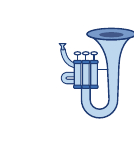
\begin{tikzpicture}[x=1mm, y=1mm, line cap=round, line join=round, baseline={([yshift=-0.6ex]current bounding box.center)}]
  % main tuning slide (left of the valves)
  \draw[eutube=0.44mm] (2.0,5.8) -- (1.0,5.8) arc[start angle=90, end angle=270, radius=0.44] -- (2.0,4.92);
  % leadpipe and mouthpiece
  \draw[eutube=0.44mm] (2.0,6.95) .. controls (1.15,7.15) and (0.65,7.9) .. (0.5,8.95);
  \filldraw[fill=eulight, draw=eunavy, line width=0.38pt] (0.33,8.95) -- (0.67,8.95) -- (0.58,9.42) -- (0.88,9.74) -- (0.02,9.74) -- (0.29,9.42) -- cycle;
  % body: left tube, bottom bow, conical bell stem and bell, one outline
  \filldraw[fill=eulight, draw=eunavy, line width=0.5pt]
    (2.85,4.3) -- (2.85,2.6) arc[start angle=180, end angle=360, radius=2.3]
    -- (7.6,6.8) .. controls (7.7,9.2) and (8.5,10.35) .. (9.75,10.95)
    arc[start angle=0, end angle=-180, x radius=3.1, y radius=0.72]
    .. controls (4.8,10.35) and (5.95,9.2) .. (6.15,6.8) -- (6.35,2.6)
    arc[start angle=360, end angle=180, radius=1.2] -- (3.95,4.3) -- cycle;
  % bell opening
  \filldraw[fill=eumid!70, draw=eunavy, line width=0.5pt] (6.65,10.95) ellipse[x radius=3.1, y radius=0.72];
  \fill[eunavy!85] (6.65,10.86) ellipse[x radius=1.55, y radius=0.33];
  % brace between the valves and the bell stem
  \draw[eunavy, line width=0.42pt] (4.87,6.4) -- (6.2,6.4);
  % three piston valves: casings, caps, stems and finger buttons
  \foreach \x in {2.35, 3.4, 4.45} {
    \filldraw[fill=eulight, draw=eunavy, line width=0.42pt, rounded corners=0.12mm] (\x-0.42,4.35) rectangle (\x+0.42,7.3);
    \filldraw[fill=eumid, draw=eunavy, line width=0.38pt, rounded corners=0.1mm] (\x-0.5,4.05) rectangle (\x+0.5,4.45);
    \filldraw[fill=eumid, draw=eunavy, line width=0.38pt, rounded corners=0.1mm] (\x-0.5,7.2) rectangle (\x+0.5,7.6);
    \draw[eunavy, line width=0.5pt] (\x,7.6) -- (\x,8.35);
    \filldraw[fill=white, draw=eunavy, line width=0.42pt] (\x,8.5) ellipse[x radius=0.43, y radius=0.2];
  }
\end{tikzpicture}}
   % \euphoniumicon: the mark left of the title

\begin{document}
\title{\begin{tabular}[c]{@{}c@{}}\raisebox{2.7pt}{\scalebox{0.75}{\euphoniumicon}}\hspace{1.2mm}\textbf{Euphonium：}\\[3pt]%
  \textbf{拡散モデルの自己回転尤度比による分布外検知}\end{tabular}}
\affiliate{sfc}{慶應義塾大学 総合政策学部3年}
\affiliate{ntt}{NTTコミュニケーション科学研究所}
\affiliate{sfc2}{慶應義塾大学院 政策・メディア研究科1年}
\author{表 紘太朗}{}{sfc}[kotaro3150@keio.jp]
\author{水谷 伸}{}{ntt}[]
\author{尾崎 慶次郎}{}{sfc2}[]
\maketitle

\section*{概要}
拡散モデルの尤度は単純な分布外画像に高い値をとり,分布外検知に失敗する(尤度パラドックス).%
提案手法 Euphonium は,画像と回転画像の尤度の比(自己回転尤度比)を検知に用いる.%
回転は複雑さを変えないため比では複雑さが消え,「正立のほうがもっともらしいか」という知識だけが残る.%
これは正立と回転を見分けるベイズ最適分類器の対数オッズであり,回転予測による手がかりを追加学習なしに密度から得る.%
推定では同じノイズを回転して両方に加え,予測誤差の差を足す(共有ノイズ推定).%
検知は, $90^\circ$ 回転の2つのスケールと $180^\circ$ 回転の1つのスケールでの誤差の対数比を足す, 1枚\nfeG{}回の順伝播のスコア $\Eu$ で行う.%
推定量と厳密な比の順位相関は\rhoEstMin{}--\rhoEstMax{}だが, $\Eu$ 自体は\rhoGMin{}--\rhoGMax{}で,別の重みづけの統計量である. %
CIFAR-10を分布内とする9集合の平均AUROCは尤度の\tabMeanNLL\%,比較手法の最良\bestBaseCten\%に対し $\Eu$ は\tabMeanG\%である.
\section{はじめに}
分布外の入力を見分けることは,機械学習モデルを安全に運用するための基本的な課題である.%
生成モデルは画像の確率密度 $p(\vec{x})$ を学習するので,尤度の低い画像を分布外とみなせばラベルなしで検知できるはずであり,拡散モデル~\cite{song2021score,karras2022edm}では確率フロー常微分方程式(PF-ODE)で対数尤度を計算できる.

ところが深層生成モデルは,分布外の画像に分布内より高い尤度を与えることがあり~\cite{nalisnick2019deep},尤度パラドックスと呼ばれる. %
CIFAR-10(一般物体の写真)のモデルはSVHN(番地の数字)により高い尤度を与え,本研究の再現でも尤度によるSVHNの検知のAUROCは\nllSVHN\%であった(チャンスレベルは50\%).%
主な原因は画像の複雑さである~\cite{serra2020input}：対数尤度は符号長に負号をつけたものなので,平坦で単純な画像ほど高くなる.

本研究は,回転した画像そのものを参照に用いる.%
回転しても画素の値の集まりも隣り合う画素の関係も変わらないため,画像と回転画像の複雑さはほぼ等しく,両者の尤度の比では複雑さが打ち消されて「正立のほうがもっともらしいか」というモデルの知識だけが残る.%
この手がかり自体は,回転を当てる分類器を学習して用いる分布外検知~\cite{golan2018geometric,hendrycks2019ss,tack2020csi}と同じであり,新しいのは,それを追加学習なしで密度から取り出すことと,同じノイズに対する二乗誤差の差(尤度比の被積分関数)として推定することである.%
本稿では, (1) 自己回転尤度比の定義,複雑さの打ち消し,ベイズ最適な回転予測器の対数オッズとしての意味,平均の符号を決める恒等式(\ref{sec:def}節), (2) 比を画像と回転画像のノイズ予測誤差の差の積分として書き,両者に同じノイズを回転して加える推定法(共有ノイズ推定)と, 1枚\nfeG{}回の順伝播のスコア Euphonium(\ref{sec:est}, \ref{sec:G}節), (3) 推定量とEuphoniumの厳密な比との照合, 8つの比較手法と符号を捨てた統計量との比較, 6つの分布内での一般性と限界(\ref{sec:exp}節)を報告する.

\section{先行研究と本研究の立ち位置}
\label{sec:related}
\begin{table}[t]\centering\footnotesize\setlength{\tabcolsep}{2.5pt}
\caption{先行研究と本研究の立ち位置(文献は本文). 測る量：検知に用いる統計量. 符号：統計量が「どちらの向き(条件)がもっともらしいか」の向きをもつか(もたない量は「大きいほど分布外」と読む). ただし符号の有無そのものの寄与は小さく(\ref{sec:exp}節の表~\ref{tab:sign}), GEPCとの違いは測る量(同じノイズに対する誤差の差か,予測差のノルムか)にある.}
\label{tab:related}
\begin{tabular}{@{}>{\raggedright\arraybackslash}p{38mm}>{\raggedright\arraybackslash}p{66mm}c>{\raggedright\arraybackslash}p{24mm}@{}}\toprule
手法 & 測る量 & 符号 & 学習\\\midrule
IC, TT & 尤度の補正(符号長,典型性) & なし & 不要\\\addlinespace[1pt]
MSMA, DiffPath, EigenScore & 拡散モデルの統計量の大きさ(分布内で較正) & なし & 不要\\\addlinespace[1pt]
GEPC & 変換した入力との予測差のノルム(分布内で較正) & なし & 不要\\\midrule
回転予測 & 回転予測の分類器の確信度 & あり & 分類器\\\addlinespace[1pt]
拡散分類器 & 条件間の予測誤差の差(同じノイズ) & あり & 条件つきモデル\\\midrule
本研究 & 回転画像との尤度比：同じノイズに対する誤差の差(\nfeG{}回の順伝播) & あり & 不要\\\bottomrule
\end{tabular}
\end{table}
\textbf{尤度の補正.}
尤度パラドックスへの対策として,モデルの符号長からPNGなどの汎用圧縮器の符号長を差し引く入力複雑さの補正(IC)~\cite{serra2020input}や,尤度がモデル自身の典型集合から外れた入力を分布外とみなす典型性検定(TT)~\cite{nalisnick2019typ}がある.

\textbf{拡散モデルの統計量.}
拡散モデルに固有の量を用いる方法として,複数のノイズの大きさでのスコアのノルムを用いるMSMA~\cite{mahmood2021msma}(本稿ではそのマハラノビス距離をMSMA型と呼ぶ),軌跡の速度と曲率を用いるDiffPath~\cite{heng2024diffpath},事後共分散の固有値を用いるEigenScore~\cite{shoushtari2026eigenscore},変換に対する予測の不整合の大きさを測るGEPC~\cite{alexis2026gepc}がある.いずれも量の大きさを測り,「どちらの向きがもっともらしいか」という符号をもたない. %
GEPCは回転したノイズ画像をノイズ除去器に通し,予測を逆回転して正立の予測と比べる点で本研究と同じ構成をとるが,予測差のノルムを「大きいほど分布外」と読む. 本研究との違いは,符号の有無そのものより(符号の寄与は小さい. \ref{sec:exp}節),同じノイズに対する誤差の差(尤度比の被積分関数)を測るか予測差のノルムを測るかにある.

\textbf{回転予測と拡散分類器.}
符号をもつ手がかりは,幾何変換を当てる分類器を自己教師ありで学習し,その確信度で分布外を検知する一連の研究~\cite{golan2018geometric,hendrycks2019ss,tack2020csi}にある(表~\ref{tab:related}).自己回転尤度比はこの手がかりの2クラス版のベイズ最適な対数オッズであり(\ref{sec:def}節),本研究はそれを追加学習なしに密度から取り出す.%
条件ごとのノイズ予測誤差を同じノイズで比べる拡散分類器~\cite{li2023dc,chen2024robust}も,同じノイズで測った誤差の差をとることで差の揺らぎを下げる.本研究は無条件のモデルで入力そのものを回転するためノイズも一緒に回転し(\ref{sec:est}節),同じノイズに対する誤差の差をとる.これが尤度比の被積分関数になる.


\section{提案手法：Euphonium}
\label{sec:method}
\subsection{定義と複雑さの打ち消し}
\label{sec:def}
\begin{figure}[t]\centering
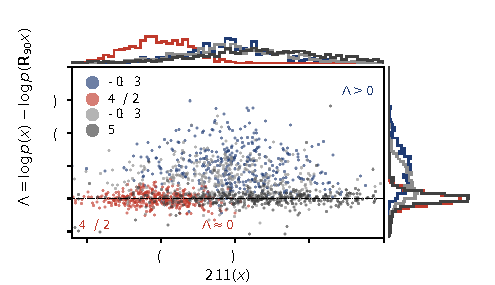
\includegraphics[width=0.5\textwidth]{figs/fig_concept.pdf}
\caption{尤度は複雑さに支配され,回転画像との比は向きに支配される(CIFAR-10の拡散モデル, PF-ODEによる尤度). 横軸は負の対数尤度(NLL, bits/dim),縦軸は $\Lambda=\log p(\vec{x})-\log p(\Rot{90}\vec{x})$.}
\label{fig:concept}
\end{figure}
画像を $\vec{x}\in\R^D$($D$ は画素値の個数),回転を直交な置換行列 $\mT$ とする($\mT\vec{x}$ は $\vec{x}$ を回した画像. $\mT^{-1}=\mT^{\top}$ であり,長さを変えない：$|\mT\vec{v}|=|\vec{v}|$). %
分布内の画像の密度(拡散モデルが学習したもの)を $p$ とし,自己回転尤度比を
\begin{equation}
\Lambda_{\mT}(\vec{x})=\log p(\vec{x})-\log p(\mT\vec{x})
\label{eq:lambda}
\end{equation}
と定義する.

\textbf{複雑さの打ち消し.}
Serr\`{a}ら~\cite{serra2020input}によれば,対数尤度は汎用の可逆圧縮(PNGなど)による符号長 $L(\vec{x})$(ビット)を用いて
\begin{equation}
\log p(\vec{x})\approx-L(\vec{x})\log2+s(\vec{x})
\label{eq:serra}
\end{equation}
と分解できる($\log2$ はビットを自然対数の単位に直す係数). %
第1項は「単純な画像ほど尤度が高い」という複雑さの効果そのものであり,分布内らしさを表すのは残りの $s(\vec{x})$ である. %
回転は画素値の集まりも隣り合う画素の関係も変えないので,符号長 $L$ をほぼ変えない. よって式~\eqref{eq:serra}を $\vec{x}$ と $\mT\vec{x}$ について引き算すると第1項が消え,
\begin{equation}
\Lambda_{\mT}(\vec{x})\approx s(\vec{x})-s(\mT\vec{x})
\label{eq:cancel}
\end{equation}
となる. %
図~\ref{fig:concept}にCIFAR-10のモデルでの実際の値を示す. %
単純なSVHNの画像は尤度ではCIFAR-10の画像より分布内らしく見えるが,回転しても尤度はほとんど変わらず $\Lambda\approx0$ である(中央値は分布内 $\lamMedID$, SVHN $\lamMedSVHN$ bits/dim).

\textbf{回転予測としての意味.}
分布内の画像 $\vec{y}$($\vec{y}\sim p$)を逆向きに回した画像 $\vec{x}=\mT^{-1}\vec{y}$ の分布を $q$ とする. %
$\vec{x}$ を $\mT$ で回せば $\vec{y}=\mT\vec{x}$ に戻り,回転は体積を変えない($|\det\mT|=1$)ので
\begin{equation}
q(\vec{x})=p(\mT\vec{x})
\label{eq:q}
\end{equation}
である. %
いま「正立($\vec{x}\sim p$)か回転($\vec{x}\sim q$)か」を当てる2クラス問題を考え, 2つのクラスが同じ確率 $1/2$ で現れるとする. %
画像 $\vec{x}$ を見たとき,正立である確率と回転である確率の比(事後オッズ)はベイズの定理より
\begin{align}
\frac{P(\text{正立}\mid\vec{x})}{P(\text{回転}\mid\vec{x})}&=\frac{\tfrac12\,p(\vec{x})}{\tfrac12\,q(\vec{x})}\notag\\
&=\frac{p(\vec{x})}{p(\mT\vec{x})}
\label{eq:bayes}
\end{align}
であり,この対数が $\Lambda_{\mT}(\vec{x})$ である. %
つまり $\Lambda_{\mT}$ は,正立と回転を見分ける最良(ベイズ最適)の分類器が出す対数オッズそのものである.

\textbf{平均の符号.}
$\Lambda_{\mT}$ が平均としてどちらの符号をとるかは,任意の密度 $p'$(分布内でも分布外でもよい)について成り立つ恒等式
\begin{equation}
\E_{\vec{x}\sim p'}[\Lambda_{\mT}(\vec{x})]=\KL(p'\,\|\,q)-\KL(p'\,\|\,p)
\label{eq:prop}
\end{equation}
で表せる. ここで $\KL(p'\,\|\,r)=\E_{\vec{x}\sim p'}[\log p'(\vec{x})-\log r(\vec{x})]$ は,分布 $p'$ から見た分布 $r$ との隔たり(カルバック・ライブラー情報量)で,常に $\KL\ge0$,等号は $p'=r$ のときに限る. %
証明：式~\eqref{eq:q}により $p(\mT\vec{x})=q(\vec{x})$ と書き,右辺に $\log p'(\vec{x})$ を足して引くと
\begin{align}
\E_{\vec{x}\sim p'}[\Lambda_{\mT}(\vec{x})]&=\E_{\vec{x}\sim p'}[\log p(\vec{x})-\log q(\vec{x})]\notag\\
&=\E_{\vec{x}\sim p'}\big[\{\log p'(\vec{x})-\log q(\vec{x})\}-\{\log p'(\vec{x})-\log p(\vec{x})\}\big]\notag\\
&=\KL(p'\,\|\,q)-\KL(p'\,\|\,p)
\label{eq:proof}
\end{align}
となる. 2行目の第1の $\{\ \}$ の期待値が $\KL(p'\,\|\,q)$,第2の $\{\ \}$ の期待値が $\KL(p'\,\|\,p)$ である(証明終). %
分布内の画像($p'=p$)では第2項が $\KL(p\,\|\,p)=0$ なので
\begin{equation}
\E_{\vec{x}\sim p}[\Lambda_{\mT}(\vec{x})]=\KL(p\,\|\,q)\ge0
\label{eq:idmean}
\end{equation}
であり,等号は回転しても分布が変わらない($p=q$)ときに限る. %
つまり分布内のデータが向きをもつ限り $\Lambda_{\mT}$ は平均として正になる(この $\KL(p\,\|\,q)$ が「向きの強さ」である). %
一方,分布外の $p'$ では式~\eqref{eq:prop}の2つの項がどちらも正になりうるので,右辺の符号は決まらない. %
分布外のほうが分布内より強い向きをもつ(回転で分布が大きく変わる)ときは右辺が式~\eqref{eq:idmean}を上回り,分布内と分布外の平均の大小が入れ替わる(\ref{sec:exp}節ではAUROCが50\%を下回った).

\subsection{共有ノイズによる推定}
\label{sec:est}
% Figure 2 (Section 3.2): the shared-noise estimate of the self-rotation likelihood ratio. Image: CIFAR-10 test 3535 (a dog), noised with sigma = 0.3 for visibility, T = R90 (figs/sh_*.pdf: paper/gen/mk_thumbs.py). The values in the caption are the macros sh* of numbers.tex (the coarsest atom of the rule, (R90, sigma_7)).
\begin{figure*}[t]\centering
\begin{adjustbox}{max width=\textwidth}
\begin{tikzpicture}[font=\footnotesize,>={Stealth[length=1.6mm]},
  img/.style={inner sep=0pt,draw=black!40},
  box/.style={draw,rounded corners=2pt,align=center,inner sep=2.5pt,minimum height=7mm,fill=white},
  res/.style={draw,rounded corners=2pt,align=center,inner sep=2.5pt,minimum height=7mm,fill=firstblue!45},
  key/.style={draw,rounded corners=2pt,align=left,inner sep=4pt,text width=49mm,minimum height=22mm,font=\footnotesize,fill=white},
  lab/.style={font=\scriptsize,align=center},
  stg/.style={font=\scriptsize\bfseries,fill=white,inner sep=1.5pt}]
% ================================================================ the computation at one noise scale sigma
% inputs
\node[img] (x) at (0,0.75) {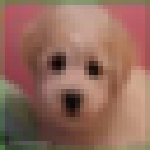
\includegraphics[width=1.1cm]{figs/sh_x.pdf}};
\node[lab,below=1pt of x] {画像 $\vec{x}$};
\node[img] (e) at (0,-1.45) {
\includegraphics[width=1.1cm]{figs/sh_eps.pdf}};
\node[lab,below=1pt of e] {ノイズ $\veps\sim\mathcal{N}(\vec{0},\mI)$};
\node[img] (xs) at (2.9,-0.35) {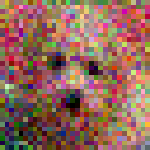
\includegraphics[width=1.1cm]{figs/sh_xs.pdf}};
\node[lab,below=1pt of xs] {$\vec{x}_\sigma=\vec{x}+\sigma\veps$};
\draw[->] (x.east) -- ($(xs.west)+(0,0.3)$);
\draw[->] (e.east) -- ($(xs.west)+(0,-0.3)$);
% upright branch
\node[box] (d1) at (6.6,0.75) {ノイズ除去器\\$\epsth(\cdot,\sigma)$};
\draw[->] ($(xs.east)+(0,0.3)$) -- ++(0.45,0) |- node[pos=0.72,above,lab] {そのまま} (d1.west);
\node[box] (b) at (10.0,0.75) {正立の予測ノイズ\\$\vec{b}=\epsth(\vec{x}_\sigma)$};
\draw[->] (d1) -- (b);
% rotated branch
\node[img] (txs) at (6.6,-1.95) {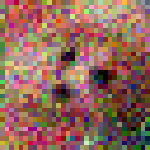
\includegraphics[width=1.1cm]{figs/sh_txs.pdf}};
\node[lab,below=1pt of txs] {$\mT\vec{x}_\sigma=\mT\vec{x}+\sigma \mT\veps$};
\draw[->] ($(xs.east)+(0,-0.3)$) -- ++(0.45,0) |- node[pos=0.74,below,lab] {回転 $\mT=\Rot{90}$} (txs.west);
\node[box] (d2) at (9.7,-1.95) {ノイズ除去器\\$\epsth(\cdot,\sigma)$};
\draw[->] (txs) -- (d2);
\node[box] (a) at (14.2,-1.95) {逆回転した予測ノイズ\\$\vec{a}=\mT^{-1}\epsth(\mT\vec{x}_\sigma)$};
\draw[->] (d2) -- node[above=1pt,lab] {逆回転\\$\mT^{-1}$} (a);
% comparison
\node[box,thick] (cmp) at (14.2,-0.3) {同じ $\veps$ と比較\\正立の誤差 $|\veps-\vec{b}|^2$\\回転の誤差 $|\veps-\vec{a}|^2$};
\draw[->] (b.east) -- ++(0.5,0) |- ($(cmp.west)+(0,0.3)$);
\draw[->] (a.north) -- (cmp.south);
% sum over the atoms (the rule: rule.json, macros of numbers.tex)
\node[res] (G) at (18.7,-0.3) {原子 $(\mT,\sigma_k)$ ごとに繰り返し,\\対数比を足す(\ruleNatoms{} 個. \nfeG{} 回の順伝播)\\[1pt]$\displaystyle \Eu=\ruleSumText$\\[1pt]$\Eu$ が大きい $\Rightarrow$ 正立のほうが\\もっともらしい $\Rightarrow$ 分布内};
\draw[->] (cmp) -- node[above,lab] {差} (G);
% step labels
\node[stg] at (0,1.75) {1. 同じノイズを加える};
\node[stg] at (7.6,1.75) {2. 正立と回転の両方を除去器に通す};
\node[stg] at (14.2,1.75) {3. 同じ $\veps$ に対する誤差を比べる};
\node[stg] at (18.7,1.75) {4. 原子で足す};
\end{tikzpicture}
\end{adjustbox}
\caption{自己回転尤度比の共有ノイズ推定とEuphoniumのスコア $\Eu$ の計算(画像はCIFAR-10の犬, $\mT=\Rot{90}$. 図のノイズ画像は見やすさのため $\sigma=0.3$). 正立の画像に用いたノイズ画像 $\vec{x}_\sigma$ をそのまま回転して通し,予測を逆回転して同じ $\veps$ と比べる. $\mT\vec{x}_\sigma$ は回転した画像に回転したノイズ $\mT\veps$ を加えたものに等しく, $\mT\veps$ は $\veps$ と同じ分布に従うため,この手順は回転画像の誤差 $e_\sigma(\mT\vec{x})$ の推定として正しい[式~\eqref{eq:shared}]. この犬の値：原子 $(\Rot{90},\sigma_7)$,すなわち $\sigma_7=\shSigma$ で $e(\vec{x})=\shEDog$, $e(\mT\vec{x})=\shETDog$(画素あたり. 対数比 $\shLRDog$), \ruleNatoms{}つの原子の対数比の和 $\Eu=\shGDog$. $\Rot{180}$ の原子も同じ手順で計算する.}
\label{fig:shared}
\end{figure*}

\textbf{尤度比を予測誤差で書く.}
拡散モデルは,ノイズ画像 $\vec{x}+\sigma\veps$($\veps\sim\mathcal{N}(\vec{0},\mI)$ はガウスノイズ, $\sigma>0$ はその大きさ)からノイズ $\veps$ を予測するノイズ除去器 $\epsth(\cdot,\sigma)$ として用いる. %
画像 $\vec{x}$ でのノイズ予測誤差(ノイズについての期待値)を
\begin{equation}
e_\sigma(\vec{x})=\E_{\veps}\big[\,|\veps-\epsth(\vec{x}+\sigma\veps,\sigma)|^2\big]
\label{eq:err}
\end{equation}
とおく. 最適なノイズ除去器に対して,対数尤度はこの誤差を $\sigma$ について積分した形に書ける~\cite{kong2023itd}：
\begin{equation}
\log p(\vec{x})=-\tfrac D2\log(2\pi e)+\!\int_0^\infty\!\big[\tfrac{D}{1+\sigma^2}-e_\sigma(\vec{x})\big]\dd\log\sigma
\label{eq:immse}
\end{equation}
($\dd\log\sigma=\dd\sigma/\sigma$. 細かいスケールも粗いスケールも対数の目盛りで等しく数える). %
式~\eqref{eq:immse}を $\vec{x}$ と $\mT\vec{x}$ のそれぞれについて書き,引き算する. 第1項と $D/(1+\sigma^2)$ の項は $\vec{x}$ によらないので消え,
\begin{equation}
\Lambda_{\mT}(\vec{x})=\int_0^\infty\big[e_\sigma(\mT\vec{x})-e_\sigma(\vec{x})\big]\dd\log\sigma
\label{eq:llr}
\end{equation}
を得る. 正立の画像のほうが回転した画像よりノイズを正確に予測できる($e_\sigma(\vec{x})<e_\sigma(\mT\vec{x})$)スケールが多いほど, $\Lambda_{\mT}$ は大きい.

\textbf{同じノイズで測る.}
式~\eqref{eq:llr}を使うには,期待値 $e_\sigma(\vec{x})$ と $e_\sigma(\mT\vec{x})$ を有限個(本稿では各スケール1個)のノイズで近似する. %
2つの誤差を別々に引いたノイズで測ると,各誤差に含まれる $|\veps|^2$ の揺らぎ(標準偏差 $\sqrt{2D}$. CIFARの画像では約78)が,細かいスケールでの2つの誤差の差(約50)より大きく,差が揺らぎに埋もれる. %
そこで2つの誤差を同じノイズ $\veps$ で測り,差をとるときに $|\veps|^2$ が打ち消されるようにしたい. %
ただし比べるのは2つの異なる入力 $\vec{x}$ と $\mT\vec{x}$ なので,同じ $\veps$ を両方に加えてもノイズ画像は同じにならない. %
鍵は, $\mT$ が直交行列なので $\mT\veps$ も $\veps$ と同じ分布 $\mathcal{N}(\vec{0},\mI)$ に従うことである(平均は $\vec{0}$,共分散は $\mT\mI\mT^{\top}=\mI$). %
したがって $e_\sigma(\mT\vec{x})$ の定義でノイズを $\veps$ から $\mT\veps$ に置き換えても期待値は変わらない. 正立の画像のノイズ画像を
\begin{equation}
\vec{x}_\sigma=\vec{x}+\sigma\veps
\label{eq:xs}
\end{equation}
とおくと, $\mT\vec{x}+\sigma\mT\veps=\mT\vec{x}_\sigma$ であるから
\begin{align}
e_\sigma(\mT\vec{x})&=\E_{\veps}\big[\,|\mT\veps-\epsth(\mT\vec{x}_\sigma,\sigma)|^2\big]\notag\\
&=\E_{\veps}\big[\,|\veps-\mT^{-1}\epsth(\mT\vec{x}_\sigma,\sigma)|^2\big]
\label{eq:shared}
\end{align}
を得る. 2行目では $|\mT\vec{v}|=|\vec{v}|$ を $\vec{v}=\veps-\mT^{-1}\epsth(\mT\vec{x}_\sigma,\sigma)$ に使った. %
つまり,正立の画像に用いたノイズ画像 $\vec{x}_\sigma$ をそのまま回転してノイズ除去器に入力し,出てきた予測を逆回転して,正立の枝と同じ $\veps$ と比較すればよい(図~\ref{fig:shared}). %
回転の枝の予測を $\vec{a}=\mT^{-1}\epsth(\mT\vec{x}_\sigma,\sigma)$,正立の枝の予測を $\vec{b}=\epsth(\vec{x}_\sigma,\sigma)$ とおくと, 1つのノイズでの2つの誤差の差は
\begin{align}
|\veps-\vec{a}|^2-|\veps-\vec{b}|^2&=|\vec{a}|^2-|\vec{b}|^2-2\veps\cdot(\vec{a}-\vec{b})\notag\\
&=(\vec{a}-\vec{b})\cdot(\vec{a}+\vec{b}-2\veps)
\label{eq:diff}
\end{align}
となる($|\veps-\vec{a}|^2=|\veps|^2-2\veps\cdot\vec{a}+|\vec{a}|^2$ と展開して引いた). %
$|\veps|^2$ の項は消え,揺らぐのは $\vec{a}-\vec{b}$(回転に対する予測のずれ)に比例する分だけである.

\begin{table*}[t]\centering\scriptsize\setlength{\tabcolsep}{4pt}\renewcommand{\arraystretch}{0.88}
\caption{比較手法との比較(AUROC, \%). 左：CIFAR-10を分布内とする9つの自然画像の分布外集合と平均. 右：ほかの5つの分布内での自然画像の分布外集合(順に9, 9, 9, 7, 4集合)の平均. $\dagger$：8つの比較手法の最良. \colorbox{firstblue}{\textbf{水色の太字}}：Oursが比較手法の最良に並ぶか上回る列(0.05ポイント以内は同点). \underline{下線}：最良にだけ下回る列(2位). Ours：式~\eqref{eq:G}のEuphonium. Ablation：PF-ODEによる厳密な $\Lambda_{90}$(印はつけない).}
\label{tab:cifar10}
\makebox[\textwidth][c]{\begin{adjustbox}{max width=1.2\textwidth}
\begin{tabular}{@{}lcccccccccc|ccccc@{}}\toprule
 & \multicolumn{10}{c|}{分布内：CIFAR-10(分布外の集合ごと)} & \multicolumn{5}{c}{分布内を変えた場合(平均)}\\
手法 & SVHN & Textures & CelebA & Tiny-IN & LSUN & ImageNet & ImageNet32 & Places365 & CIFAR-100 & 平均 & SVHN & CelebA & CIFAR-100 & ImageNet-64 & FashionMNIST\\\midrule
% written by paper/gen/make_paper.py: left, AUROC (%) on the nine CIFAR-10 sets and their mean; right, mean AUROC over the natural OOD sets of the other five IDs
NLL(尤度) & 12.5 & 62.3 & 61.3 & 49.1 & 72.1 & 58.6 & 76.9 & 69.7 & 50.2 & 57.0 & 98.9 & 81.6 & 56.4 & 54.7 & 33.1\\
IC (PNG) & 81.7 & 74.7 & 65.8 & 48.6 & 83.7$^{\dagger}$ & 76.7 & 83.0 & 82.6$^{\dagger}$ & 55.7 & 72.5 & 92.7 & 86.7 & 67.1$^{\dagger}$ & 49.8 & 87.3\\
IC (J2K) & 96.0 & 74.1 & 67.7$^{\dagger}$ & 45.9 & 77.8 & 72.0 & 74.2 & 77.4 & 54.4 & 71.1 & 75.5 & 81.5 & 66.3 & 47.0 & 40.0\\
TT & 73.6 & 66.2 & 39.9 & 47.4 & 61.6 & 59.0 & 73.7 & 63.1 & 54.7 & 59.9 & 98.6 & 84.9 & 54.2 & 57.4 & 62.1\\
MSMA 型 & 91.1 & 90.1$^{\dagger}$ & 43.7 & 71.5 & 48.4 & 59.0 & 70.4 & 52.4 & 54.5 & 64.6 & 99.0 & 99.6 & 59.1 & 62.4$^{\dagger}$ & 95.8$^{\dagger}$\\
DiffPath & 99.4$^{\dagger}$ & 85.3 & 39.4 & 77.4$^{\dagger}$ & 62.4 & 73.6 & 84.3$^{\dagger}$ & 65.3 & 60.3 & 71.9 & 99.5$^{\dagger}$ & 99.8$^{\dagger}$ & 63.2 & 55.3 & 81.3\\
GEPC & 84.7 & 66.0 & 28.9 & 50.9 & 35.0 & 47.2 & 47.2 & 41.1 & 49.7 & 50.1 & 91.8 & 98.7 & 55.5 & 49.1 & 84.0\\
EigenScore & 66.8 & 72.1 & 61.4 & 76.9 & 83.6 & 79.3$^{\dagger}$ & 78.2 & 80.9 & 76.1$^{\dagger}$ & 75.0$^{\dagger}$ & 86.1 & 86.1 & 44.9 & 44.1 & 93.5\\
\midrule
Ours：Euphonium(10 回) & 94.9 & \cellcolor{firstblue}\textbf{94.8} & \cellcolor{firstblue}\textbf{91.7} & \cellcolor{firstblue}\textbf{93.8} & \cellcolor{firstblue}\textbf{92.2} & \cellcolor{firstblue}\textbf{93.5} & \cellcolor{firstblue}\textbf{92.4} & \cellcolor{firstblue}\textbf{91.6} & \cellcolor{firstblue}\textbf{76.0} & \cellcolor{firstblue}\textbf{91.2} & 98.0 & \cellcolor{firstblue}\textbf{100.0} & \cellcolor{firstblue}\textbf{72.8} & \underline{60.5} & \cellcolor{firstblue}\textbf{98.9}\\
Ablation：厳密な比 $\Lambda_{90}$(512 回) & 95.9 & 94.6 & 94.8 & 93.5 & 90.3 & 91.8 & 89.9 & 89.7 & 71.1 & 90.2 & 89.6 & -- & 73.0 & 62.6 & --\\\bottomrule

\end{tabular}
\end{adjustbox}}
\end{table*}
\subsection{Euphonium：\nfeG{}回の順伝播の向きの統計量}
\label{sec:G}
\textbf{積分を和にする.}
ノイズの大きさを, $\log\sigma$ について等間隔な格子 $\sigma_k=0.01\times3162.3^{(k-1)/15}$($k=1,2,\dots$. 隣との間隔は $h=0.537$)にとり,式~\eqref{eq:llr}の積分を幅 $h$ の長方形の和で近似する. 用いるのは細かい側の10点, $\sigma_1=0.01$ から $\sigma_{10}=\sigTen$ まで(この窓の決め方は後述). %
スケール $\sigma_k$ での $e_{\sigma_k}$ の推定値[式~\eqref{eq:shared}を1つのノイズで近似したもの]を $\hat e_k$ と書くと
\begin{align}
\Lambda_{\mT}(\vec{x})&\approx h\sum_{k=1}^{10}\big[\hat e_k(\mT\vec{x})-\hat e_k(\vec{x})\big]\notag\\
&\approx h\sum_{k=1}^{10}\hat e_k(\vec{x})\log\frac{\hat e_k(\mT\vec{x})}{\hat e_k(\vec{x})}
\label{eq:disc}
\end{align}
となる. 2つ目の近似は,差を $\hat e_k(\mT\vec{x})-\hat e_k(\vec{x})=\hat e_k(\vec{x})\,u_k$($u_k$ は相対的な差)と書き, $|u|$ が小さいときの $u\approx\log(1+u)$ を使って $u_k\approx\log\{\hat e_k(\mT\vec{x})/\hat e_k(\vec{x})\}$ としたものである. %
ノイズは,スケールごとに1つの $\veps$ を引いて $+\veps$ と $-\veps$ の両方で評価して平均し(符号反転対),すべてのテスト画像に同じノイズを用いる.

\textbf{重みを外す.}
式~\eqref{eq:disc}の右辺は,スケール $k$ の対数比 $\log\{\hat e_k(\mT\vec{x})/\hat e_k(\vec{x})\}$ に重み $\hat e_k(\vec{x})$ をかけて足したものである. %
この重みとその揺らぎは細かいスケールほど大きい($\sigma_1$ では平均 $0.52D$, $\sigma_{10}$ では $0.02D$)ので,細かいスケールの項が和を支配する. %
そこで検知には,重みを外して対数比だけを足した向きの統計量を用いる. 回転 $\mT$ とスケール $k$ の組を原子と呼び,用いる原子の集合を $\mathcal A$ として
\begin{equation}
\Eu(\vec{x})=\ruleSumText
\label{eq:G}
\end{equation}
\begin{equation}
\mathcal A=\ruleAtomsText
\label{eq:atoms}
\end{equation}
とする(\ruleAtomsWords). %
正立の画像は $\mathcal A$ に現れる\ruleNscale{}つのスケールで $\pm\veps$ の計\ruleNfeUp{}回,回転画像は\ruleNatoms{}つの原子ごとに $\pm\veps$ の計\ruleNfeRot{}回,合わせて1枚\nfeG{}回の順伝播である. %
これが提案手法 Euphonium のスコアである(本文と表では Euphonium,式では $\Eu$ と書く). %
Euphonium は $\Lambda_{\mT}$ の推定値ではない. 各原子の証拠を画像ごとの誤差 $\hat e_k(\vec{x})$ で割って正規化し,等しい重みで足した別の統計量であり,式~\eqref{eq:llr}の積分の格子のうち証拠のあるスケールだけを2つの回転について用いる(\ref{sec:exp}節で両者を分けて検証する).

\textbf{各スケールの符号.}
式~\eqref{eq:prop}は積分全体についての主張だが,各スケールの項 $e_\sigma(\mT\vec{x})-e_\sigma(\vec{x})$ も,分布内の画像で平均すればすべての $\sigma$ で非負である. 理由は次のとおり. %
$\E_{\vec{x}\sim p}[e_\sigma(\vec{x})]$ は,分布 $p$ の画像にノイズを加えたものから $\veps$ を当てるときの,最良の推定器($p$ に最適な $\epsth$)の誤差,すなわち最小誤差である. %
一方 $\E_{\vec{x}\sim p}[e_\sigma(\mT\vec{x})]$ は,回転した画像(分布 $q$)に同じ $\epsth$ を使ったときの誤差であり, $q$ に合わせた最良の推定器の誤差($q$ の最小誤差)以上である. %
$\mT$ が直交でノイズが等方的なので,問題全体を $\mT$ で回しても何も変わらず, $q$ の最小誤差は $p$ の最小誤差に等しい. よって $\E_{\vec{x}\sim p}[e_\sigma(\mT\vec{x})]\ge\E_{\vec{x}\sim p}[e_\sigma(\vec{x})]$ である. %
したがってスケールの一部だけを足しても,分布内での平均の符号は保たれる[対数比では近似的. 補足資料の図~\ref{fig:G}(b)で確かめる].

\textbf{構成の決め方.}
原子の集合 $\mathcal A$ は,主評価に含まれない分布外データセット(STL-10, GTSRB, EuroSATなど11集合)と分布内の開発用画像でのAUROCの6つの分布内での平均を基準に選び,主評価のデータは用いていない. %
候補は,回転 $\Rot{90}$, $\Rot{180}$, $\Rot{270}$ とスケール $\sigma_1$--$\sigma_{10}$ の原子を1枚\nfeG{}回以内で組み合わせた\nCandTwo{}通りすべてで,式~\eqref{eq:atoms}はその最良(\selMean\%)である(0.1ポイント以内は同点とし,同点の中では順伝播が少なく,最も弱い分布内の平均が高いものを採る. 補足資料のA.4). %
対数比の形[式~\eqref{eq:disc}の第2の近似]は,細かいスケールの重みを外すという上の理由による設計上の選択であり,選択用データで選んだものではない. 誤差の差の形[同じ式の第1の近似]で同じ探索をすると,選択用データでは\selDiffBest\%と対数比の形を上回り,主評価では\diffBestMain\%と下回る(補足資料のA.4). %
$\sigma_{11}$--$\sigma_{13}$ の原子は,候補に加えても選択用データの上位に入らない(A.4). 逆伝播は用いない.

\section{実験と結果}
\label{sec:exp}
\begin{figure}[t]\centering
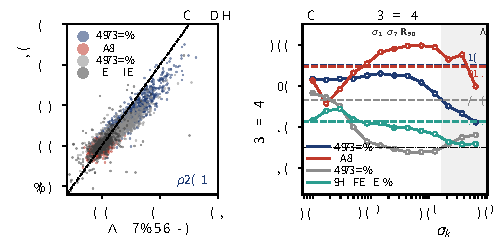
\includegraphics[width=0.6\textwidth]{figs/fig_verify.pdf}
\caption{推定量と Euphonium をそれぞれ厳密な比と照合する($\mT=\Rot{90}$). (a) 10スケールの共有ノイズ推定[式~\eqref{eq:disc}の第1の近似, 40回]とPF-ODEによる厳密な $\Lambda$(512回. CIFAR-10のモデル). 推定は $\sigma\le\sigTen$ の和なので値は小さいが順位は保たれる. (b) スケールごとの対数比 $\log\hat e_k(\Rot{90}\vec{x})/\hat e_k(\vec{x})$ のAUROC(自然画像の分布外集合の平均. 13スケール, 4つの分布内). 塗りつぶした点が Euphonium の用いる原子[\ruleAtomsWords. $\Rot{180}$ の対数比は補足資料の図~\ref{fig:G}(b)に示す]($\sigma_{11}$--$\sigma_{13}$ は Euphonium にも推定量にも用いない),破線は厳密な $\Lambda$ のAUROC.}
\label{fig:verify}
\end{figure}
\textbf{設定.}
分布内データは6つで, FashionMNIST以外は公開の学習済み拡散モデルをそのまま使った(補足資料の表~\ref{tab:models}).%
主な実験はCIFAR-10のEDM~\cite{karras2022edm}(VP, DDPM++)で行う.%
比較手法は尤度(NLL)と\ref{sec:related}節の手法の計8つ(ICはPNGとJPEG2000を別に数える)で,公式のコードまたは論文の手順に従い,同じモデルと同じ画像で評価した.当てはめには開発用,評価には最終評価用の画像を使い, PF-ODEを用いる手法は1集合あたり1000枚(ImageNet-64は500枚)で評価した.

\textbf{推定の検証：推定量と Euphonium を分けて照合する.}
式~\eqref{eq:llr}の被積分関数は,分布内のCIFAR-10ではすべてのスケールで正, SVHNとTexturesでは0に近い[補足資料の図~\ref{fig:G}(a)]. %
10スケールの共有ノイズ推定(40回)と厳密な比の順位相関は,厳密な比を計算した4つの分布内データセットの分布内画像で\rhoEstMin{}(\rhoEstMinName)--\rhoEstMax{}[CIFAR-10. 図~\ref{fig:verify}(a)]であり,推定は厳密な比の順位をおおむね再現する(ノイズを独立に引くと, CIFAR-10を分布内とする12組の平均AUROCが\estMain\%から\estIndep\%に下がる. 補足資料の表~\ref{tab:controls}).%
一方,検知に用いる Euphonium 自体と厳密な比の順位相関は分布内画像で\rhoGMin{}--\rhoGMax{},分布内と分布外を合わせても\rhoPoolGMin{}--\rhoPoolGMax{}にとどまる(補足資料の図~\ref{fig:gode}).%
理由は図~\ref{fig:verify}(b)にある. %
対数比の証拠は分布内ごとに別のスケールにあり, SVHN(数字)では粗いスケール($\sigma_9$ で\psCoarseSVHN\%, $\sigma_1$ では\psFineSVHN\%), CIFAR-100では細かいスケール($\sigma_1$ で\psFineCh\%, $\sigma_5$, $\sigma_7$, $\sigma_9$ では約50\%)にある.%
差の形[図~\ref{fig:verify}(a)の推定量]は厳密な比の順位を保ち,平均AUROCも厳密な比の側に寄る(CIFAR-100で\dTenCh\%, SVHNで\dTenSVHN\%).%
対数比はこれを画像ごとの誤差 $\hat e_k(\vec{x})$ で正規化するので,誤差の小さい単純な画像では差が増幅され,スケール間の重みも等しくなる.そのためSVHNを分布内とする平均は Euphonium の\oGSVHN\%に対し厳密な比では\oODESVHN\%である. CIFAR-100では,証拠のない粗いスケールまで等しく足した $\Rot{90}$ の10スケールの対数比の和は\gTenCh\%と厳密な比(\oODECh\%)を大きく下回るが, Euphonium は証拠のある $\sigma_1$ に原子を置くため\oGCh\%と厳密な比に並ぶ(補足資料の表~\ref{tab:scale}). %
粗い3スケール($\sigma=\sigDropA$--$\sigDropC$)の対数比のAUROCはCIFAR-10で\psDropACten{}--\psDropCCten\%と低く, 10スケールの和に加えると平均が\gTenCten\%から\gThirteenCten\%に下がる(補足資料の表~\ref{tab:scale}). 開発用の分割で決めた $\sigma\le\sigTen$ の窓はこれと整合する(事後の確認. $\sigma\gg1$ では向きの情報が残らない).

\begin{table}[t]\centering\scriptsize\setlength{\tabcolsep}{4pt}\renewcommand{\arraystretch}{0.9}
\caption{符号か大きさか：自然画像の分布外集合での平均AUROC(\%). Euphonium と $-|\Eu|$ は同じ\nfeG{}回の評価から. 最終列はGEPCの実行(GEPCの6つのノイズレベルすべて. 本研究のスケールとは異なる)の $\Rot{90}$ の予測差 $\|\vec a-\vec b\|^2/\|\vec b\|^2$ を「大きいほど分布外」と読んだもの. 全列は補足資料の表~\ref{tab:signfull}.}
\label{tab:sign}
\begin{tabular}{@{}lccc@{}}\toprule
分布内 & \signColsText\\\midrule
% written by paper/gen/make_paper.py: sign or magnitude (Table 3; rows = IDs, columns = statistics; mean AUROC over the natural OOD sets)
CIFAR-10 & \cellcolor{firstblue}91.2 & 9.9 & 28.8\\
SVHN & \cellcolor{firstblue}98.0 & 5.4 & 96.0\\
CelebA & \cellcolor{firstblue}100.0 & 0.0 & 1.3\\
CIFAR-100 & \cellcolor{firstblue}72.8 & 29.3 & 47.1\\
ImageNet-64 & \cellcolor{firstblue}60.5 & 39.0 & 52.7\\
FashionMNIST & \cellcolor{firstblue}98.9 & 4.0 & 13.7\\
平均 & \cellcolor{firstblue}86.9 & 14.6 & 39.9\\\bottomrule

\end{tabular}
\end{table}
\textbf{比較手法との比較.}
表~\ref{tab:cifar10}に9つの分布外集合でのAUROCを示す. %
尤度(NLL)の平均は\tabMeanNLL\%で, SVHNでは\nllSVHN\%である. %
Euphonium は平均\tabMeanG\%で, 9つの集合すべてで尤度を上回る. %
比較手法の最良は\bestBaseNameCten{}の\bestBaseCten\%であり, Euphonium は9つのうち\winsCten{}つの集合で比較手法の最良に並ぶか上回り,残るSVHNではDiffPathの\dpSVHN\%, IC (J2K)の\icjSVHN\%に対し\GSVHN\%(\GrankSVHN{}位)である.%
厳密な比 $\Lambda_{90}$(512回)の平均は\tabMeanODE\%で \nfeG{}回の Euphonium と同等だが,集合ごとには異なる. %
なお,同じモデルのノイズ除去器の特徴による分布内の学習画像へのkNN~\cite{sun2022knn}(特徴の最近傍. 本稿の比較手法には含めず,最終発表で扱う)はCIFAR-10で\knnCten\%, 6つの分布内の平均で\knnMeanSix\%であり, Euphonium 単独は\knnLoseN{}つの分布内でこれに及ばない. 本稿の「比較手法の最良」は公表された8つの手法の中での最良を指す.

\textbf{符号か大きさか.}
表~\ref{tab:sign}に,同じ\nfeG{}回の評価から符号を捨てた統計量を示す. %
$-|\Eu|$ の平均AUROCはCIFAR-10で\signMabsGCten\%, 6つの分布内の平均で\signMabsGMean\%と50\%を大きく下回る.回転に対する予測の不整合は分布内の正立画像でこそ大きく, SVHNやTexturesのような分布外の画像では回転しても誤差が変わらないからである[補足資料の図~\ref{fig:G}(a)].%
したがって読み方を反転した $|\Eu|$ は Euphonium に近く(6つの平均で\signAbsFlipMean\%),画像ごとの符号の寄与は小さく,効いているのは不整合の向き(分布内で大きい)である.符号が効くのは分布外のほうが強い向きをもつ組で,そこでは Euphonium も $|\Eu|$ も反転し(CIFAR-100に対するCIFAR-10で Euphonium は\oWorstGCh\%),「大きいほど分布外」の読み方が当たる(\signRevChCten\%). %
GEPCの実行の $\Rot{90}$ の予測差のノルムは,分布内によって向きが変わる(表~\ref{tab:sign}の最終列).本研究とGEPCの違いは符号そのものより,同じ $\veps$ に対する誤差の差(尤度比の被積分関数)を測るかノルムを測るかにあると考えられるが,同じ\nfeG{}回の評価からの $\|\vec a_k-\vec b_k\|^2$ との対照は計算中である.

\textbf{分布内データセットを変えた場合.}
表~\ref{tab:cifar10}の右に,ほかの5つの分布内データセットでの平均を示す. %
Euphonium は6つのうち\nIDbest{}つで比較手法の最良に並ぶか上回り,全\nPairs{}組(補足資料の表~\ref{tab:all}, \ref{tab:allb})では\winsAll{}組で並ぶか上回り, \secondAll{}組で2位であった.%
下回るのは\idLoseList{}である. SVHNでは尤度だけで\oNLLSVHN\%に達し,比較手法の最良(\oBestNameSVHN)の\oBestSVHN\%に対し Euphonium は\oGSVHN\%である[$\Rot{180}$ の原子は数字では弱い(補足資料のA.4). $\Rot{90}$ だけの構成(A.4の c3)なら\prevSVHNmean\%]. %
向きの弱いCIFAR-100とImageNet-64($\overline{\Eu}$ が\gbarCh{}と\gbarIN. 補足資料の表~\ref{tab:orient})では Euphonium は\oGCh\%, \oGIN\%で,前者は比較手法の最良(\oBestCh\%)を上回り,後者は下回る(\oBestIN\%).%
平均を下げているのは\revText{}のように分布外のほうが強い向きをもつ組であり,式~\eqref{eq:prop}の片側性のとおり反転は厳密な比でも起こる(\oWorstODECh\%, \oWorstODEIN\%).%
向きの弱さがデータの性質か学習不足かを分けるため, CIFAR-10とCIFAR-100の両方のモデルで両方の画像を評価した(補足資料の表~\ref{tab:cross}).%
どちらのモデルでもCIFAR-10の画像の $\overline{\Eu}$ は\crossGCtenCten{}と\crossGChCten{}, CIFAR-100の画像は\crossGCtenCh{}と\crossGChCh{}であり(厳密な比でも同じ),差はモデルではなく画像の側にあり,反転の主因は学習量ではなくデータの性質と考えられる(補足資料のA.7. ImageNet-64に対するCelebAも $\overline{\Eu}$ が\gbarINCel{}対\gbarIN{}と分布外のほうが大きい).

\section{今後の課題}
回転との比は片側の判定であり,分布外のほうが強い向きをもつ組で反転する.今後は,学習した回転分類器との直接の比較に加え,反転する条件を分布内の画像だけから見積もる方法,分布内ごとに異なる証拠のスケール[図~\ref{fig:verify}(b)]の重みを開発用画像だけから決める方法,同じ\nfeG{}回の評価から得る向きによらない統計量で反転を補う規則を検討する.

\bibliographystyle{miru2025j-unsrt}   % numbered in order of citation: miru2025j.bst without SORT (paper/README.md)
\bibliography{refs}

\clearpage
\section*{補足資料}
\renewcommand{\thetable}{A\arabic{table}}\setcounter{table}{0}
\renewcommand{\thefigure}{A\arabic{figure}}\setcounter{figure}{0}

\subsection*{A.1\quad 実験の設定}
\begin{table}[h]\centering\footnotesize\setlength{\tabcolsep}{3pt}
\caption{分布内データセットと拡散モデル. 5つは公開されている学習済みの重みを変更せずに用いた.}
\label{tab:models}
\begin{adjustbox}{max width=\columnwidth}
\begin{tabular}{@{}llll@{}}\toprule
分布内 & 解像度 & モデル & 出典\\\midrule
CIFAR-10 & $32{\times}32$ & EDM(VP, DDPM++) & \cite{karras2022edm}\\
CIFAR-100 & $32{\times}32$ & EDMの前処理によるDDPM++ & \cite{chen2024robust}\\
SVHN & $32{\times}32$ & VP-SDE & \cite{kamkari2024geometric}\\
CelebA & $32{\times}32$ & iDDPM & \cite{nichol2021improved}\\
ImageNet-64 & $64{\times}64$ & EDM2-XS(条件なし) & \cite{karras2024edm2}\\
FashionMNIST & $32{\times}32$ & EDMの前処理によるU-Net & 本研究で学習\\
\bottomrule\end{tabular}
\end{adjustbox}
\end{table}
分布外集合は, $32{\times}32$ の分布内データセットに対しては他の自然画像のデータセット[CIFAR-10/100, SVHN, CelebA, Textures(DTD), Tiny-ImageNet(検証画像を $32{\times}32$ に縮小), LSUNとImageNet(CSI~\cite{tack2020csi}が配布するリサイズ版), ImageNet32(ダウンサンプル版の検証画像), Places365(検証画像)], ImageNet-64に対してはOpenOOD v1.5~\cite{zhang2023openood}の集合(SSB-hard, NINCO, iNaturalist, Textures, OpenImage-O)とPlaces365, CelebA, FashionMNISTに対しては $32{\times}32$ に埋め込んだ灰色画像の集合(MNIST, KMNIST, Omniglot, notMNIST)である.%
さらに各分布内データセットについてその画像を上下反転した集合を加え, ImageNet-64以外には一様ノイズと定数画像も加えた(計\nPairs{}組).%
上下反転した分布内の画像は,内容は分布内と同じで向きだけが異なる集合であり,向きの手がかりを直接評価する. %
Euphonium は分布内の開発用画像には依存しないが,ノイズの乱数はすべての画像で共通にした. %
Euphonium の構成(回転,スケール,ノイズの引き方)は主評価に含まれないデータだけで選んだ(A.4).%
比較手法の当てはめには分布内の開発用画像を用いた. %
MSMA型は, 20スケールでのスコアの大きさのベクトルの,分布内の開発用画像に対するマハラノビス距離である. %
DiffPath, GEPC, EigenScoreは公式のコードに従って再実装した：DiffPathはDDIM 10段の軌跡の6次元の統計量にガウス混合を当てはめる. GEPCは6変換(左右・上下反転, $\Rot{90}$, $\Rot{180}$, 縦・横1画素の巡回シフト)の予測差を公開設定のノイズレベルで測り(CIFAR-10, SVHN, CelebAは各自の公開設定, CIFAR-100, ImageNet-64, FashionMNISTにはCIFAR-10の設定. レベルの選択と密度推定は分布内の開発用画像で行う), EigenScoreは5つの時刻での事後共分散の上位3固有値を分布内でz化して足す. %
PF-ODEを用いる手法(NLL, IC, TT, $\Lambda_{90}$. 厳密な尤度はHeun法64段で順伝播と逆伝播を128回ずつ,比はその2倍の計512回)は1集合あたり1000枚(ImageNet-64は500枚)で評価し,合成画像の集合では計算していない. 厳密な $\Lambda_{90}$ はCIFAR-10, SVHN, CIFAR-100, ImageNet-64の4つの分布内で計算し(CelebAとFashionMNISTでは計算していない),上下反転の集合でも計算していない. %
DiffPathとGEPCの再実装は,論文の設定(32$\times$32の全分布内に1つのCelebAモデル)では論文に載る6組の公表値をほぼ再現する(公表値との差はDiffPathで最大3.1ポイント, GEPCは公式コードの時刻の扱いで最大3.9ポイント). EigenScoreは公式コードがなく,論文の9組の平均92.5\%に対し再実装は79.5\%で,モデルの違い(本稿は各分布内の公開モデル,論文は1つのCelebAモデル)と論文が指定しない設定によると考えられる.%
本文の表の値はすべての手法が共通にもつ画像(各集合1000枚, ImageNet-64は500枚,合成画像は2000枚)で計算した. 「自然画像の分布外集合」は上下反転と合成画像を除いた分布外集合を指す(FashionMNISTの灰色画像の集合を含む).

\subsection*{A.2\quad 計算量と処理時間}
\begin{table}[h]\centering\footnotesize\setlength{\tabcolsep}{4pt}
\caption{1枚あたりの計算量と処理時間(CIFAR-10のモデル, EDM DDPM++, 5600万パラメータ). NFE：順伝播の回数, VJP：逆伝播(ベクトルとヤコビ行列の積)の回数. TFLOPは1回の順伝播42.4 GFLOP,順伝播と逆伝播の組85.1 GFLOPの実測から. CPU時間はすべての行を同じ2コアのCPUで1回のセッションの中で測定した(fp32, 4枚ずつのバッチ, 同じ構造のネットワークで重みは乱数. 計算量は重みによらない. 時間はほぼすべてネットワークの評価で, Euphonium の集計は無視できる). IC の時間は尤度の計算に PNG / JPEG 2000 の符号長の計算(1枚0.002秒)が加わる. GPU(GeForce RTX 2080 Ti, fp16, 500枚ずつ)では20回の構成(c3)の評価が1枚\gpuBU{}ミリ秒だった(Euphonium の GPU 時間は未計測. 順伝播の回数は c3 の半分). 水色の行がOurs.}
\label{tab:cost}
\begin{adjustbox}{max width=\columnwidth}
\begin{tabular}{@{}lcccc@{}}\toprule
手法 & NFE & VJP & TFLOP & CPU 秒/枚\\\midrule
DiffPath & 10 & 0 & 0.42 & 2.2\\
\cellcolor{firstblue}Ours：Euphonium(\nfeG{}回の順伝播) & \cellcolor{firstblue}\nfeG & \cellcolor{firstblue}0 & \cellcolor{firstblue}0.42 & \cellcolor{firstblue}2.1\\
GEPC & 14 & 0 & 0.59 & 3.1\\
Ablation：格子の候補 c3($\Rot{90}$, 5スケール. A.4) & 20 & 0 & 0.85 & 4.3\\
MSMA 型 & 20 & 0 & 0.85 & 4.3\\
Ablation：$\Rot{90}+\Rot{180}$, 10スケール(A.4の r60) & 60 & 0 & 2.54 & 13.1\\
EigenScore & 180 & 0 & 7.63 & 40.3\\
NLL, TT, IC (PNG / J2K) & 128 & 128 & 10.89 & 59.9\\
Ablation：厳密な比 $\Lambda_{90}$(PF-ODE) & 256 & 256 & 21.79 & 115.2\\
\bottomrule\end{tabular}
\end{adjustbox}
\end{table}
Euphonium は1枚あたり\nfeG{}回の順伝播(0.42 TFLOP)で計算でき,逆伝播を用いないため推論専用の環境でも動作する(表~\ref{tab:cost}). %
PF-ODEによる尤度(NLL, TT, IC)は順伝播と逆伝播を128回ずつ要し,厳密な自己回転尤度比はその2倍である.

\subsection*{A.3\quad 向きの統計量 Euphonium の中身}
図~\ref{fig:G}(a)は式~\eqref{eq:llr}の被積分関数,(b)は式~\eqref{eq:G}の対数比を $\Rot{90}$ と $\Rot{180}$ についてスケールごとに示し, Euphonium の用いる\ruleNatoms{}つの原子[式~\eqref{eq:atoms}]を印で示したものである.%
図~\ref{fig:G}(c)は\ruleNatoms{}つの対数比の和 Euphonium の分布で,分布内の画像の\GposID\%で $\Eu>0$ である一方, SVHNの中央値は $\GmedSVHN$ である.

\subsection*{A.4\quad 規則の選択とAblation：主評価に含まれないデータだけで選ぶ}
\label{sec:variants}
\begin{table}[h]\centering\footnotesize
\caption{Euphonium の構成の選択(上)と格子の候補のAblation(下). 選ばれた構成が Ours(水色の行). 上：原子(回転,スケール)の集合. 回転は $\Rot{90}$, $\Rot{180}$, $\Rot{270}$,スケールは $\sigma_1$--$\sigma_{10}$,ノイズは符号反転対(対)で, \nfeG{}回以内の\nCandTwo{}通りのうち選択用データで上位の3つ(e10, e10b, e10c)と,予算を8, 6, 4回に絞ったときの最良(e8, e6, e4. 参考). 下：向きに共通のスケールの格子を用いる候補. 格子 $\sigma_1,\dots,\sigma_{10}$ を1つおきに間引いたもの(奇：$\{\sigma_1,\sigma_3,\sigma_5,\sigma_7,\sigma_9\}$,偶：$\{\sigma_2,\dots,\sigma_{10}\}$),3つおき,または全10点で,ノイズは対か $+\veps$ だけ(単). c1--c12は20回以内, r60, r80は10スケールすべてを用いる60回と80回の構成, devは主評価と同じ分布外データセットの開発用の複製で候補を選ぶとどうなるかを示す参考値(採用しない). 「選択」：分布内の開発用画像と主評価に含まれない分布外データセット[32$\times$32の4モデルではSTL-10, GTSRB, Flowers-102, EuroSAT, MNIST, Oxford-IIIT Pet, Caltech-101, Food-101, FGVC-Aircraft, Imagenette, Rendered SST-2. ImageNet-64は同じ集合の64$\times$64版(Imagenetteを除く10集合), FashionMNISTは灰色の文字・数字・自然画像の6集合]でのAUROCの6つの分布内での平均(この列で選ぶ). 「主評価」：採用後に計算した自然画像の分布外集合でのAUROCの6つの分布内での平均と,全\nPairs{}組のうち比較手法の最良に並ぶか上回った組の数(選択には用いていない).}
\label{tab:variants}
\begin{adjustbox}{max width=\columnwidth}
\setlength{\tabcolsep}{3pt}\begin{tabular}{@{}lllcrccc@{}}\toprule
 & 向き & スケール & ノイズ & NFE & 選択 & 主評価 & 勝ち数\\\midrule
% written by paper/gen/make_paper.py: Euphonium candidates (PROTOCOL_10NFE.md, top) and the grid candidates (Ablation, PROTOCOL_20NFE.md, bottom): mean AUROC (%) on the selection data and on the main evaluation, pairs won
\cellcolor{firstblue}\textbf{Ours}(e10) & \cellcolor{firstblue}$\Rot{90}$, $\Rot{180}$ & \cellcolor{firstblue}$\Rot{90}$：$\{\sigma_{1},\sigma_{7}\}$; $\Rot{180}$：$\{\sigma_{1}\}$ & \cellcolor{firstblue}対 & \cellcolor{firstblue}10 & \cellcolor{firstblue}85.7 & \cellcolor{firstblue}86.9 & \cellcolor{firstblue}34\\
参考(e10b) & $\Rot{90}$, $\Rot{180}$ & $\Rot{90}$：$\{\sigma_{1},\sigma_{6}\}$; $\Rot{180}$：$\{\sigma_{1}\}$ & 対 & 10 & 85.7 & 87.5 & 36\\
参考(e10c) & $\Rot{90}$, $\Rot{180}$, $\Rot{270}$ & $\Rot{90}$：$\{\sigma_{1}\}$; $\Rot{180}$：$\{\sigma_{1}\}$; $\Rot{270}$：$\{\sigma_{6}\}$ & 対 & 10 & 85.7 & 87.5 & 37\\
参考(e8) & $\Rot{90}$, $\Rot{180}$ & $\Rot{90}$：$\{\sigma_{6}\}$; $\Rot{180}$：$\{\sigma_{1}\}$ & 対 & 8 & 84.1 & 86.4 & 34\\
参考(e6) & $\Rot{90}$, $\Rot{180}$ & $\Rot{90}$：$\{\sigma_{1}\}$; $\Rot{180}$：$\{\sigma_{1}\}$ & 対 & 6 & 82.2 & 82.3 & 30\\
参考(e4) & $\Rot{90}$ & $\Rot{90}$：$\{\sigma_{1}\}$ & 対 & 4 & 81.6 & 81.7 & 27\\
\midrule
Ablation(c1) & $\Rot{180}$ & 1 つおき(奇) & 対 & 20 & 82.1 & 85.6 & 33\\
Ablation(c2) & $\Rot{180}$ & 1 つおき(偶) & 対 & 20 & 80.5 & 84.9 & 33\\
Ablation(c3) & $\Rot{90}$ & 1 つおき(奇) & 対 & 20 & 83.9 & 85.4 & 36\\
Ablation(c4) & $\Rot{90}$ & 1 つおき(偶) & 対 & 20 & 82.7 & 84.4 & 38\\
Ablation(c5) & $\Rot{90}$, $\Rot{180}$ & $\{\sigma_{1},\sigma_{5},\sigma_{9}\}$ & 対 & 18 & 83.7 & 85.7 & 35\\
Ablation(c6) & $\Rot{90}$, $\Rot{180}$ & $\{\sigma_{2},\sigma_{6},\sigma_{10}\}$ & 対 & 18 & 82.9 & 84.8 & 35\\
Ablation(c7) & $\Rot{180}$ & 10 点すべて & 単 & 20 & 81.1 & 85.2 & 34\\
Ablation(c8) & $\Rot{90}$ & 10 点すべて & 単 & 20 & 83.1 & 84.8 & 39\\
Ablation(c9) & $\Rot{90}$, $\Rot{180}$ & 1 つおき(奇) & 単 & 15 & 83.7 & 85.6 & 36\\
Ablation(c10) & $\Rot{90}$, $\Rot{180}$ & 1 つおき(偶) & 単 & 15 & 82.4 & 84.5 & 34\\
Ablation(c11) & $\Rot{90}$, $\Rot{180}$, $\Rot{270}$ & 1 つおき(奇) & 単 & 20 & 83.6 & 85.5 & 36\\
Ablation(c12) & $\Rot{90}$, $\Rot{180}$, $\Rot{270}$ & 1 つおき(偶) & 単 & 20 & 82.5 & 84.5 & 34\\
Ablation(r60) & $\Rot{90}$, $\Rot{180}$ & 10 点すべて & 対 & 60 & 84.4 & 86.6 & 43\\
Ablation(r80) & $\Rot{90}$, $\Rot{180}$, $\Rot{270}$ & 10 点すべて & 対 & 80 & 84.1 & 86.3 & 44\\
Ablation(dev) & $\Rot{180}$ & $\{\sigma_1,\sigma_3,\sigma_4,\sigma_6,\sigma_8\}$ & 対 & 20 & -- & 86.4 & 35\\\bottomrule

\end{tabular}
\end{adjustbox}
\end{table}
表~\ref{tab:variants}に候補と結果を示す.%
候補の比較に主評価の分布外データセット(とその開発用の複製)は用いていない(選択用のImagenetteはImageNetの10クラスの部分集合で,主評価のImageNet32・ImageNetと出典が重なるが画像は別である).%

\textbf{原子の集合の選択.}
候補は対の原子の集合に限った($+\veps$ だけの候補や対との混合は,別の乱数の実行の値を足し合わせることになるため除いた). %
上位の3つ(e10, e10b, e10c)は\selMeanTwo, \selSecondTwo, \selThirdTwo\%で0.1ポイント以内の同点であり,順伝播もすべて\nfeG{}回なので,最も弱い分布内の平均(\selMinNew, \selMinSecond, \selMinThird\%)が最も高い e10 を採用した. %
この同点の規則は,上位2つの順位が計算に用いる開発用画像の集合(全画像か, $+\veps$ だけの実行とも共通の画像か)によって入れ替わることがわかった時点で定めたものである. どの候補を採っても主評価の結論は変わらない(e10b は主評価\secondMainMean\%で\secondWins{}組, e10c は\thirdMainMean\%で\thirdWins{}組). %
選択用の分布外集合を交互に2分割し,片方で候補を選んでもう片方で確かめても,どちらの分割でも選ばれた構成は格子の候補の最良(c3)を上回った(88.0対87.7, 83.0対80.6). %
この探索は,格子の候補(下段)の主評価を見たあとに行ったが,選択には主評価のデータを一切用いていない.

\textbf{対数比の形とスケールの範囲.}
対数比の形[式~\eqref{eq:disc}の第2の近似]は\ref{sec:G}節の理由による設計上の選択であり,選択用データで選んだものではない. 同じ候補の族を誤差の差の形(第1の近似)で評価すると,選択用データでの最良は\diffBestCand(\selDiffBest\%. 最も弱い分布内は\selDiffBestMin\%)で,対数比の形の\selMean\%を上回る. 主評価では\diffBestMain\%(\diffBestWins{}組)で, Euphonium の\meanSixG\%(\winsAll{}組)を平均で下回り, SVHNを分布内とする平均が\diffBestSVHN\%に下がる(対数比は誤差の小さい単純な画像で差を増幅する. \ref{sec:exp}節). Euphonium と同じ3つの原子を差の形で足した「差Eu」(表~\ref{tab:scale})は主評価\dEuMain\%(\dEuWins{}組. 6つの分布内のうち\dEuIDbest{}つで比較手法の最良に並ぶか上回る)で,下がるのはSVHN(\dEuSVHN\%)だけである. %
スケールの範囲は,候補を $\sigma_{13}=\sigDropC$ までの原子に広げても(FashionMNISTの開発用の実行は10スケールまでのため,ほかの5つの分布内で)上位10候補に $\sigma_{11}$--$\sigma_{13}$ の原子は入らない(対数比・差のどちらの形でも). %
当初,対数比の形と $\sigma\le\sigTen$ の窓は,最終評価用の画像を開く前に主評価と同じ分布外データセットの開発用の複製で決めていた. これは主評価に含まれないデータだけで選ぶという本稿の規則に反するため,上のとおり選択用データで確かめ直した：窓の結論は同じで,対数比の形は選択用データでは支持されない.

\textbf{Ablation：格子の候補と順伝播の回数.}
向きに共通のスケールの格子を用いる20回以内の12候補(c1--c12. 分布内の分布が左右対称なら $\Rot{270}$ は $\Rot{90}$ と, $\Rot{180}$ は上下反転と同じ証拠をもつため,回転は $\Rot{90}$ と $\Rot{180}$ とその組とし,参考として $\Rot{270}$ を加えた候補も載せる)の選択用データでの最良は c3($\Rot{90}$,奇の5点,対)の\selMeanPrev\%で, 2--4位(c9, c5, c11)との差は0.3ポイント程度である. 主評価では12候補は84.4--85.7\%の範囲にあり, c3 は\prevMainMean\%(\prevWins{}組)で, Euphonium(\meanSixG\%, \winsAll{}組)に平均で及ばない(並ぶか上回る組の数はやや多い). %
$\Rot{180}$ だけを用いる候補(c1, c2, c7)はSVHNを分布内とするときに選択用データで大きく下がる(c1で85.7\%. c3は\selPrevSVHN\%).%
数字は $180^\circ$ 回しても別の数字(6と9)か同じ数字(0, 8)に見えるが, $90^\circ$ 回すと数字に見えないためと考えられる. Euphonium も $\Rot{180}$ の原子をもつため, SVHNでは c3 より下がり(選択用データで\selNewSVHN\%対\selPrevSVHN\%,主評価で\oGSVHN\%対\prevSVHNmean\%), CIFAR-100では細かいスケール $\sigma_1$ の原子により上がる(主評価で\oGCh\%対\prevGCh\%).%
10スケールすべてを用いる r60(60回)と r80(80回)は主評価86.6\%, 86.3\%で,順伝播を6--8倍にしても Euphonium と同程度である. %
逆に予算を絞ると,選択用データでの最良は8回(e8)で主評価\budgetMainEight\%, 6回(e6)で\budgetMainSix\%, 4回(e4)で\budgetMainFour\%である. ノイズを $+\veps$ だけにした単一ノイズの候補(別の実行. 対と共通の画像で評価)では, 5回以内の最良は\singleFiveCand(\singleFiveNfe{}回)で選択用データ\singleFiveSel\%,主評価\singleFiveMain\%(\singleFiveWins{}組)であり,同じ画像での Euphonium(\pairOnCommonSel\%, \pairOnCommonMain\%)に選択用データで1ポイント,主評価で0.5ポイント及ばない(符号反転対の効果はA.5).

\subsection*{A.5\quad ノイズの共有の効果}
\begin{table}[h]\centering\footnotesize\setlength{\tabcolsep}{4pt}
\caption{推定の方法を変えたときの Euphonium の平均AUROC[\%. CIFAR-10を分布内とする12組(上下反転と合成画像を含む). 最終評価用のすべての画像を用いるため,本文の表(9集合,共通の部分集合)とは値が異なる]. 乱数による揺らぎの標準偏差は\estSeedSd{}ポイント.}
\label{tab:controls}
\begin{tabular}{@{}lc@{}}\toprule
推定の方法 & 平均AUROC\\\midrule
共有ノイズ,符号反転対(本文の設定) & \estMain\\
画像と回転画像に独立なノイズ & \estIndep\\
\estAltText & \estAlt\\
共有ノイズ,テスト画像ごとに別のノイズ & \estPerimg\\
\bottomrule\end{tabular}
\end{table}
\begin{table}[h]\centering\footnotesize\setlength{\tabcolsep}{3pt}
\caption{共有ノイズは差からノイズの大きさの揺らぎを取り除く(CIFAR-10のモデル, $\mT=\Rot{90}$,最終評価用の分布内の画像\varN{}枚,ノイズの乱数3通り. 二乗誤差は $D=\varDim$ 個の画素値について和をとる). スケールごとに, $e_k(\vec{x})$ の平均,差 $e_k(\Rot{90}\vec{x})-e_k(\vec{x})$ の平均,画像平均した $e_k(\vec{x})$ の乱数の間での最大のずれ($|\veps|^2$ の揺らぎ. $\sqrt{2D}=78$),画像平均した共有ノイズの差の最大のずれ,独立なノイズを用いたときの差の画像ごとの分散と共有ノイズでの差の分散を示す.}
\label{tab:variance}
\begin{adjustbox}{max width=\columnwidth}
\begin{tabular}{@{}lrrrrrr@{}}\toprule
$\sigma_k$ & $\bar e_k(\vec{x})$ & 差の平均 & $e_k(\vec{x})$ のずれ & 差のずれ & 分散(独立) & 分散(共有)\\\midrule
% written by paper/gen/make_paper.py: effect of the shared noise (R90, final-split ID images, three seeds)
0.01 & 1585 & 52.7 & 34.7 & 4.1 & 2275 & 1613\\
0.0171 & 1241 & 49.2 & 72.0 & 3.6 & 3233 & 1388\\
0.0293 & 1068 & 38.3 & 48.5 & 1.7 & 1686 & 925\\
0.0501 & 818 & 29.8 & 8.6 & 0.6 & 1209 & 522\\
0.0858 & 621 & 30.2 & 13.3 & 1.9 & 808 & 528\\
0.147 & 433 & 28.3 & 10.7 & 2.3 & 675 & 518\\
0.251 & 275 & 25.3 & 8.1 & 0.9 & 639 & 457\\
0.43 & 184 & 22.8 & 9.0 & 1.8 & 542 & 417\\
0.736 & 114 & 15.5 & 1.8 & 1.0 & 258 & 243\\
1.26 & 65 & 9.1 & 3.0 & 0.2 & 123 & 106\\\bottomrule

\end{tabular}
\end{adjustbox}
\end{table}
表~\ref{tab:controls}は,推定の方法だけを変えて Euphonium を計算したものである.%
画像と回転画像に独立なノイズを用いると平均AUROCは\estMain\%から\estIndep\%に下がり,符号反転対を除くと\estAlt\%に下がる.%
テスト画像ごとに別のノイズを用いても\estPerimg\%と変わらない.%
表~\ref{tab:variance}は,共有ノイズが差から揺らぎを取り除く様子を直接測定したものである.%
細かいスケールでは $e_k(\vec{x})$ の画像平均の乱数によるずれが最大\varDevMax{}に達し,差の平均(最大\varFineDiff)を上回りうるが,共有ノイズでの差のずれはどのスケールでも\varDevDiffMax{}以下である.画像ごとの差の分散も共有ノイズのほうが小さい(右の2列).

\clearpage\onecolumn
\makeatletter\setlength{\@fptop}{0pt}\makeatother   % float-only pages start at the top
\begin{figure*}[t]\centering
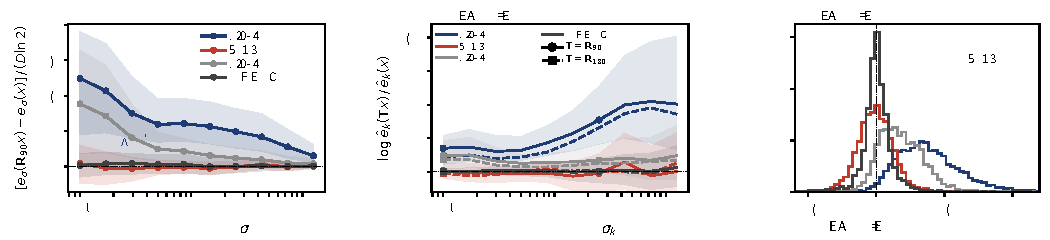
\includegraphics[width=\textwidth]{figs/fig_G.pdf}
\caption{被積分関数と向きの統計量 Euphonium(CIFAR-10のモデル,最終評価用の画像). (a) 式~\eqref{eq:llr}の被積分関数 $[e_\sigma(\Rot{90}\vec{x})-e_\sigma(\vec{x})]/(D\ln2)$ の中央値と25--75\%の範囲(10スケール). 分布内のCIFAR-10ではすべてのスケールで正であり,単純なSVHNと複雑なTexturesではどちらも0に近い. (b) スケールごとの対数比 $\log\hat e_k(\mT\vec{x})/\hat e_k(\vec{x})$ の中央値(10スケール. 実線：$\mT=\Rot{90}$,帯は25--75\%の範囲. 破線：$\mT=\Rot{180}$)と, Euphonium の用いる\ruleNatoms{}つの原子(印). 分布内の画像ではどちらの回転でもすべてのスケールで正であり,粗いスケールほど大きい. (c) \ruleNatoms{}つの対数比の和 Euphonium の分布.分布内の画像の\GposID\%で $\Eu>0$ である.}
\label{fig:G}
\end{figure*}
\subsection*{A.6\quad 符号か大きさか(全列)}
\begin{table}[h]\centering\footnotesize\setlength{\tabcolsep}{2.5pt}
\caption{表~\ref{tab:sign}の全列. 自然画像の分布外集合での平均AUROC(\%). $\ell_{\mT,k}=\log\hat e_k(\mT\vec{x})/\hat e_k(\vec{x})$ は原子 $(\mT,k)\in\mathcal A$ の対数比. Euphonium, $-|\Eu|$, $-\sum|\ell_{\mT,k}|$, $-|\Eu-\mathrm{med}|$ は同じ\nfeG{}回の評価から. 予測差(GEPC)はGEPCの実行の $\Rot{90}$ の予測差 $\|\vec a-\vec b\|^2/\|\vec b\|^2$ を「大きいほど分布外」と読んだもの, GEPCは6変換を用いる本来のGEPC(表~\ref{tab:cifar10}). 最後の列は参考：Euphonium の分布内の開発用画像の中央値 med からのずれ(両側の典型性)で,反転する組は補えるが他で下がる.}
\label{tab:signfull}
\begin{adjustbox}{max width=\columnwidth}
\begin{tabular}{@{}lcccccc@{}}\toprule
分布内 & \signAllColsText\\\midrule
% written by paper/gen/make_paper.py: sign or magnitude (Table A6; rows = IDs, columns = statistics)
CIFAR-10 & \cellcolor{firstblue}91.2 & 9.9 & 10.9 & 28.8 & 50.1 & 78.2\\
SVHN & \cellcolor{firstblue}98.0 & 5.4 & 5.8 & 96.0 & 91.8 & 85.0\\
CelebA & \cellcolor{firstblue}100.0 & 0.0 & 0.0 & 1.3 & 98.7 & 100.0\\
CIFAR-100 & \cellcolor{firstblue}72.8 & 29.3 & 26.9 & 47.1 & 55.5 & 60.4\\
ImageNet-64 & \cellcolor{firstblue}60.5 & 39.0 & 39.7 & 52.7 & 49.1 & 58.9\\
FashionMNIST & \cellcolor{firstblue}98.9 & 4.0 & 5.9 & 13.7 & 84.0 & 92.7\\
平均 & \cellcolor{firstblue}86.9 & 14.6 & 14.9 & 39.9 & 71.6 & 79.2\\\bottomrule

\end{tabular}
\end{adjustbox}
\end{table}
表~\ref{tab:signfull}に表~\ref{tab:sign}の全列を示す. 同じ\nfeG{}回の評価から符号を捨てた $-|\Eu|$ と $-\sum|\ell_{\mT,k}|$ は,分布内のほうが回転に対する不整合が大きいために6つの分布内すべてで50\%を下回る. GEPCの実行から取り出した予測差のノルムは分布内によって向きが変わる(CIFAR-10で\signGEPCrCten\%, SVHNで\signGEPCrSVHN\%). Euphonium の中央値からのずれ(両側)は反転する組を補う(CIFAR-100に対するCIFAR-10で Euphonium の\oWorstGCh\%に対し\signMtwoChCten\%)が, CIFAR-100の9集合の平均では\signMtwoCh\%と Euphonium の\oGCh\%より下がり,向きの強い分布内でも Euphonium より下がる.

\subsection*{A.7\quad 分布内データセットの向きの強さと反転}
\begin{table}[h]\centering\footnotesize\setlength{\tabcolsep}{3pt}
\caption{向きの弱さはデータの性質である：モデルと画像の交差評価. CIFAR-10のモデルとCIFAR-100のモデル(同じDDPM++の構成)で, CIFAR-10とCIFAR-100の画像(本文の表と同じ最終評価用の画像)の Euphonium の平均(括弧は平均を標準偏差で割った値)と厳密な $\Lambda_{90}$ の平均(bits/dim). 行(モデル)の差はなく,列(画像)の差だけがある.}
\label{tab:cross}
\begin{adjustbox}{max width=\columnwidth}
\begin{tabular}{@{}lcccc@{}}\toprule
 & \multicolumn{2}{c}{CIFAR-10の画像} & \multicolumn{2}{c}{CIFAR-100の画像}\\
\cmidrule(lr){2-3}\cmidrule(lr){4-5}
 & $\overline{\Eu}$ & $\bar\Lambda_{90}$ & $\overline{\Eu}$ & $\bar\Lambda_{90}$\\\midrule
% written by paper/gen/make_paper.py: model x image cross-evaluation (mean of Euphonium, d', mean exact Lambda_90 in bits/dim; final-split images)
CIFAR-10 のモデル & 0.16 (1.31) & 0.099 & 0.07 (1.09) & 0.053\\
CIFAR-100 のモデル & 0.17 (1.38) & 0.104 & 0.08 (1.19) & 0.058\\\bottomrule

\end{tabular}
\end{adjustbox}
\end{table}
\begin{table}[h]\centering\footnotesize\setlength{\tabcolsep}{3pt}
\caption{分布内の画像での Euphonium の平均 $\pm$ 標準偏差[式~\eqref{eq:prop}の向きの強さの目安],反転した組(自然画像と上下反転の集合のうち Euphonium のAUROCが49\%未満)の数, Euphonium のAUROCが最も低い分布外集合とそこでの Euphonium と厳密な比 $\Lambda_{90}$ のAUROC(\%).}
\label{tab:orient}
\begin{adjustbox}{max width=\columnwidth}
\begin{tabular}{@{}lcclcc@{}}\toprule
分布内 & $\overline{\Eu}$ & 反転 & 最も低い組 & Euphonium & $\Lambda_{90}$(ODE)\\\midrule
% written by paper/gen/make_paper.py: mean and sd of Euphonium on the ID images, number of reversed pairs, lowest pair
CIFAR-10 & 0.16 $\pm$ 0.12 & 0/10 & CIFAR-100 & 76.0 & 71.1\\
SVHN & 0.17 $\pm$ 0.08 & 0/10 & 上下反転 & 85.4 & --\\
CelebA & 0.66 $\pm$ 0.15 & 0/10 & Textures & 99.9 & --\\
CIFAR-100 & 0.08 $\pm$ 0.07 & 1/10 & CIFAR-10 & 24.4 & 29.4\\
ImageNet-64 & 0.04 $\pm$ 0.03 & 1/8 & CelebA & 6.6 & 25.2\\
FashionMNIST & 0.38 $\pm$ 0.20 & 0/5 & 上下反転 & 92.5 & --\\\bottomrule

\end{tabular}
\end{adjustbox}
\end{table}
反転が起きたのは,分布内の画像での Euphonium の平均が小さい(向きの弱い)CIFAR-100とImageNet-64に限られ,どちらも分布外のほうが強い向きをもつ組(CIFAR-10, CelebA)である.%
反転は厳密な比 $\Lambda_{90}$ でも同じ組で起こるため,推定の誤差によるものではない.%
表~\ref{tab:cross}の交差評価に加え,同じ構成と学習手順の自前のU-Netを学習量を変えて評価した(分布内の画像のみ. $\Rot{180}$, 5スケール $\{0.01, 0.029, 0.05, 0.147, 0.43\}$ の対数比の和). %
CIFAR-10では分布内の $\overline{\Eu}$ が\snapNFirstCten{}M枚の\snapFirstCten{}から\snapNLastCten{}M枚の\snapLastCten{}まで学習とともに単調に増え,一般物体の画像であるTiny-ImageNet($32{\times}32$)を学習データとするモデルでも\snapNFirstTIN{}M枚の\snapFirstTIN{}から\snapNLastTIN{}M枚の\snapLastTIN{}へとゆるやかに増える.%
向きの強さは学習とともに増えるが,同じ学習量での差はデータの側にある(8M枚で\snapEightTIN{}対\snapEightCten, \snapNLastTIN{}M枚で\snapLastTIN{}対\snapLastCten).%
なお,狭い領域のモデル(SVHN, CelebA)は自分の領域以外の画像の向きをほとんど知らず(他の9集合で $|\overline{\Eu}|\le\gbarNarrowMax$),一般物体の2つのモデル(CIFAR-10, CIFAR-100)は10集合のそれぞれに互いにほぼ同じ $\overline{\Eu}$ を与える(差は\gbarBroadDiffMax{}以内).

\subsection*{A.8\quad スケールごとの証拠と, Euphonium と厳密な比の対応}
\begin{figure}[h]\centering
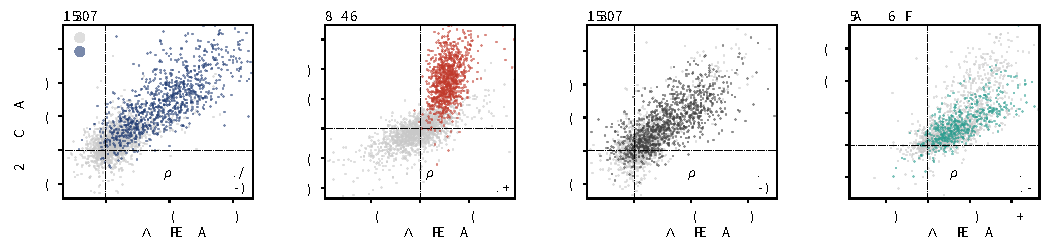
\includegraphics[width=\textwidth]{figs/fig_gode.pdf}
\caption{検知に用いる Euphonium(\nfeG{}回. 縦軸)とPF-ODEによる厳密な $\Lambda_{90}$(横軸, bits/dim)の画像ごとの対応. 厳密な比を計算した4つの分布内データセットについて,分布内の画像(色)と自然画像の分布外集合(灰色)を示す. $\rho$ は順位相関(分布内の画像のみ,および分布内と分布外を合わせたもの). Euphonium は $\Rot{180}$ の原子を含み,重みづけも $\Lambda_{90}$ と異なる. SVHNでは $\Lambda$ が小さくても Euphonium が大きい(証拠が粗いスケールにあり, $\Lambda$ はそれを軽く, Euphonium は等しく重みづける). SVHNで10スケールの推定量の順位相関も低い(\rhoEstSVHN)のは,分布内の $\Lambda$ の広がりが小さい(標準偏差 \lamSdSVHN{} bits/dim. CIFAR-10は \lamSdCten)ためと考えられる.}
\label{fig:gode}
\end{figure}
\begin{table}[h]\centering\footnotesize\setlength{\tabcolsep}{3pt}
\caption{スケールごとの対数比 $\log\hat e_k(\mT\vec{x})/\hat e_k(\vec{x})$ のAUROC(\%. 自然画像の分布外集合の平均. 本文の表と同じ最終評価用の画像)と,原子の集合を変えた和のAUROC. 分布内ごとに上の行が $\mT=\Rot{90}$,下の行[($\Rot{180}$)]が $\mT=\Rot{180}$ で,太字が Euphonium の用いる原子. 「Eu」は Euphonium(\nfeG{}回),「10」は $\Rot{90}$ の $\sigma_1$--$\sigma_{10}$ の和(40回),「13」は $\sigma_{13}=\sigDropC$ までの和. 「差Eu」「差10」は対数比ではなく誤差の差 $\hat e_k(\mT\vec{x})-\hat e_k(\vec{x})$ を同じ原子についてそのまま足した形[式~\eqref{eq:disc}の第1の近似. 差10が図~\ref{fig:verify}(a)で厳密な比と照合した推定量]. $\Lambda_{90}$ はPF-ODEの厳密な比.}
\label{tab:scale}
\makebox[\textwidth][c]{\begin{adjustbox}{max width=1.2\textwidth}
\begin{tabular}{@{}lccccccccccccccccccc@{}}\toprule
分布内 & $\sigma_1$ & $\sigma_2$ & $\sigma_3$ & $\sigma_4$ & $\sigma_5$ & $\sigma_6$ & $\sigma_7$ & $\sigma_8$ & $\sigma_9$ & $\sigma_{10}$ & $\sigma_{11}$ & $\sigma_{12}$ & $\sigma_{13}$ & Eu & 10 & 13 & 差Eu & 差10 & $\Lambda_{90}$\\
 & 0.01 & 0.017 & 0.029 & 0.05 & 0.086 & 0.147 & 0.251 & 0.43 & 0.736 & 1.26 & 2.15 & 3.69 & 6.31 & & & & & & \\\midrule
% written by paper/gen/make_paper.py: per-scale log-ratio AUROC (mean over the natural OOD sets), sums over atom sets, exact ratio
CIFAR-10 & \textbf{83.3} & 82.9 & 83.4 & 83.4 & 85.0 & 86.0 & \textbf{85.0} & 84.8 & 81.6 & 76.2 & 70.0 & 66.5 & 62.2 & 91.2 & 91.0 & 87.2 & 90.1 & 91.8 & 90.2\\
CIFAR-10($\Rot{180}$) & \textbf{83.7} & 85.7 & 85.5 & 84.8 & 85.6 & 87.3 & 86.3 & 86.1 & 83.5 & 78.0 & 69.0 & 65.0 & 56.8 &  &  &  &  &  & \\
SVHN & \textbf{82.6} & 71.4 & 78.3 & 86.4 & 90.8 & 96.3 & \textbf{98.1} & 99.4 & 99.6 & 98.8 & 92.8 & 95.2 & 79.7 & 98.0 & 99.8 & 99.7 & 73.5 & 78.2 & 89.6\\
SVHN($\Rot{180}$) & \textbf{59.5} & 57.4 & 68.6 & 75.8 & 81.9 & 84.3 & 94.7 & 94.1 & 90.6 & 88.9 & 85.9 & 73.3 & 31.0 &  &  &  &  &  & \\
CelebA & \textbf{99.9} & 99.9 & 99.8 & 99.9 & 99.9 & 99.9 & \textbf{99.8} & 99.9 & 99.8 & 99.5 & 99.7 & 98.7 & 98.8 & 100.0 & 100.0 & 100.0 & 100.0 & 100.0 & --\\
CelebA($\Rot{180}$) & \textbf{100.0} & 100.0 & 100.0 & 99.9 & 99.9 & 99.9 & 99.8 & 99.8 & 99.6 & 99.1 & 99.3 & 97.5 & 95.2 &  &  &  &  &  & \\
CIFAR-100 & \textbf{76.5} & 74.4 & 70.2 & 59.8 & 52.8 & 50.9 & \textbf{49.1} & 47.6 & 47.6 & 48.0 & 51.6 & 54.8 & 56.1 & 72.8 & 60.2 & 59.7 & 79.6 & 72.1 & 73.0\\
CIFAR-100($\Rot{180}$) & \textbf{79.8} & 78.3 & 72.3 & 60.0 & 51.5 & 51.0 & 47.4 & 48.7 & 48.8 & 49.9 & 49.7 & 52.4 & 51.6 &  &  &  &  &  & \\
ImageNet-64 & \textbf{63.2} & 67.8 & 68.7 & 63.5 & 61.7 & 61.8 & \textbf{59.5} & 59.5 & 58.0 & 56.5 & 52.7 & 51.4 & 51.7 & 60.5 & 61.7 & 59.3 & 63.8 & 62.9 & 62.6\\
ImageNet-64($\Rot{180}$) & \textbf{63.9} & 68.8 & 69.8 & 64.3 & 62.3 & 62.7 & 62.0 & 62.3 & 59.4 & 55.2 & 50.6 & 49.8 & 46.6 &  &  &  &  &  & \\
FashionMNIST & \textbf{84.4} & 89.6 & 91.6 & 96.3 & 96.2 & 97.9 & \textbf{98.7} & 98.8 & 97.9 & 97.7 & 96.6 & 89.9 & 81.1 & 98.9 & 99.7 & 99.4 & 98.9 & 99.8 & --\\
FashionMNIST($\Rot{180}$) & \textbf{75.3} & 78.5 & 84.8 & 92.2 & 92.6 & 95.6 & 96.5 & 97.4 & 97.1 & 97.7 & 96.2 & 89.8 & 66.9 &  &  &  &  &  & \\\bottomrule

\end{tabular}
\end{adjustbox}}
\end{table}
表~\ref{tab:scale}は図~\ref{fig:verify}(b)の数値である. %
CIFAR-10では $\sigma_1$--$\sigma_9$ の対数比が81--86\%でほぼ平坦であり, $\sigma_{11}$--$\sigma_{13}$ では\psDropACten{}, \psDropBCten{}, \psDropCCten\%と下がる. 13スケールの和は10スケールの和より\gTenCten{}から\gThirteenCten\%に下がる. %
SVHNでは粗いスケール($\sigma_7$--$\sigma_{10}$)の証拠が強く, CIFAR-100では証拠が細かいスケール($\sigma_1$--$\sigma_3$ で70\%以上)にほぼ限られる.%
厳密な比は式~\eqref{eq:disc}の重み $\hat e_k$ によって細かいスケールを重く数えるため, SVHNでは Euphonium より低く, CIFAR-100では $\Rot{90}$ の10スケールの等重みの和「10」(\gTenCh\%)より高い. Euphonium は CIFAR-100 の証拠を $\sigma_1$ の原子で拾うため,厳密な比に並ぶ(\oGCh\%対\oODECh\%). 対数比を差の形にすると値は厳密な比の側に動き(「差10」はSVHNで\dTenSVHN\%, CIFAR-100で\dTenCh\%. 対数比の「10」は\gTenSVHN\%, \gTenCh\%,厳密な比は\oODESVHN\%, \oODECh\%),対数比との違いが重みづけによることを示す.

\subsection*{A.9\quad 全結果}
表~\ref{tab:all}と表~\ref{tab:allb}に全\nPairs{}組の結果を示す. %
Euphonium は\winsAll{}組で8つの比較手法の最良に並ぶか上回り(0.05ポイント以内を同点), 1ポイント以内を同点とみなせば\winsAllOne{}組である.%
下回った組の多くは,尤度だけで99\%に達するSVHNを分布内とする組(11組すべて. Euphonium は\oGSVHN\%で,比較手法の最良は99\%を超える)と,向きの弱いCIFAR-100とImageNet-64を分布内とする組(13組)であり,残りはCIFAR-10に対するSVHNと, CIFAR-10・FashionMNISTに対する合成画像(一様ノイズ・定数画像)である.%
上下反転した分布内の画像(内容は分布内と同じで向きだけが異なる)は, Euphonium ではすべての分布内データセットで\vflipGlo--\vflipGhi\%で検知でき,比較手法の最良(\vflipBaseLo--\vflipBaseHi\%)に\vflipWins{}つすべてで並ぶか上回る.%
これは Euphonium が向きそのものを手がかりにしていることの直接の確認である.
\begin{table}[h]\centering\scriptsize\setlength{\tabcolsep}{3pt}\renewcommand{\arraystretch}{0.92}
\caption{全\nPairs{}組のAUROC(\%)(1/2：CIFAR-10, SVHN, CelebAを分布内とする組). 8つの比較手法, Ours：Euphonium(\ruleAtomsWords. \nfeG{}回),および2つのAblation：$\Eu_{10}$($\Rot{90}$ の10スケール $\sigma_1$--$\sigma_{10}$ の対数比の和, 40回)と厳密な $\Lambda_{90}$(PF-ODE, 512回). $\dagger$：8つの比較手法の中での最良(SOTA). \colorbox{firstblue}{\textbf{水色の太字}}：Oursが比較手法の最良に並ぶか上回る組(BEST. 2つの表で\winsAll/\nPairs{}組). \underline{下線}：Oursが比較手法の最良にだけ下回る組(2位. \secondAll{}組). Ablationには印をつけない. PF-ODEを用いる手法は合成画像の集合では計算していない(--).}
\label{tab:all}
\makebox[\textwidth][c]{\begin{adjustbox}{max width=1.2\textwidth}
\begin{tabular}{@{}llccccccccccc@{}}\toprule
分布内 & 分布外 & NLL & IC (PNG) & IC (J2K) & TT & MSMA 型 & DiffPath & GEPC & EigenScore & Euphonium (Ours) & $\Eu_{10}$ (Ablation) & $\Lambda_{90}$ (Ablation, ODE)\\\midrule
% written by paper/gen/make_paper.py: AUROC (%) on all 63 pairs; Euphonium in light-blue bold where it ties or beats the best of the eight methods
CIFAR-10 & CIFAR-100 & 50.2 & 55.7 & 54.4 & 54.7 & 54.5 & 60.3 & 49.7 & 76.1$^{\dagger}$ & \cellcolor{firstblue}\textbf{76.0} & 84.8 & 71.1\\
 & SVHN & 12.5 & 81.7 & 96.0 & 73.6 & 91.1 & 99.4$^{\dagger}$ & 84.7 & 66.8 & 94.9 & 96.4 & 95.9\\
 & CelebA & 61.3 & 65.8 & 67.7$^{\dagger}$ & 39.9 & 43.7 & 39.4 & 28.9 & 61.4 & \cellcolor{firstblue}\textbf{91.7} & 85.4 & 94.8\\
 & Textures & 62.3 & 74.7 & 74.1 & 66.2 & 90.1$^{\dagger}$ & 85.3 & 66.0 & 72.1 & \cellcolor{firstblue}\textbf{94.8} & 95.3 & 94.6\\
 & Tiny-ImageNet & 49.1 & 48.6 & 45.9 & 47.4 & 71.5 & 77.4$^{\dagger}$ & 50.9 & 76.9 & \cellcolor{firstblue}\textbf{93.8} & 92.7 & 93.5\\
 & LSUN & 72.1 & 83.7$^{\dagger}$ & 77.8 & 61.6 & 48.4 & 62.4 & 35.0 & 83.6 & \cellcolor{firstblue}\textbf{92.2} & 91.2 & 90.3\\
 & ImageNet & 58.6 & 76.7 & 72.0 & 59.0 & 59.0 & 73.6 & 47.2 & 79.3$^{\dagger}$ & \cellcolor{firstblue}\textbf{93.5} & 92.7 & 91.8\\
 & ImageNet32 & 76.9 & 83.0 & 74.2 & 73.7 & 70.4 & 84.3$^{\dagger}$ & 47.2 & 78.2 & \cellcolor{firstblue}\textbf{92.4} & 91.1 & 89.9\\
 & Places365 & 69.7 & 82.6$^{\dagger}$ & 77.4 & 63.1 & 52.4 & 65.3 & 41.1 & 80.9 & \cellcolor{firstblue}\textbf{91.6} & 89.3 & 89.7\\
 & 上下反転 & 52.7 & 53.7 & 53.5 & 50.7 & 52.3 & 54.9 & 45.2 & 78.9$^{\dagger}$ & \cellcolor{firstblue}\textbf{90.8} & 89.7 & --\\
 & 一様ノイズ & -- & -- & -- & -- & 100.0$^{\dagger}$ & 100.0$^{\dagger}$ & 60.6 & 60.5 & 97.8 & -- & --\\
 & 定数画像 & -- & -- & -- & -- & 100.0$^{\dagger}$ & 99.3 & 95.6 & 25.3 & 91.9 & -- & --\\
\midrule
SVHN & CIFAR-10 & 98.9 & 87.1 & 64.4 & 98.6 & 98.5 & 99.1$^{\dagger}$ & 92.3 & 88.4 & 98.0 & 99.9 & 88.1\\
 & CIFAR-100 & 98.5 & 89.4 & 68.7 & 97.7 & 98.4 & 99.2$^{\dagger}$ & 92.2 & 84.6 & 97.9 & 99.8 & 86.8\\
 & CelebA & 99.9$^{\dagger}$ & 88.4 & 64.1 & 99.9$^{\dagger}$ & 98.8 & 99.4 & 95.2 & 85.1 & 97.9 & 99.9 & 85.2\\
 & Textures & 96.8 & 95.2 & 80.9 & 97.0 & 99.6$^{\dagger}$ & 99.5 & 80.7 & 90.2 & 96.9 & 99.2 & 88.2\\
 & Tiny-ImageNet & 98.5 & 81.7 & 47.5 & 97.7 & 97.7 & 99.2$^{\dagger}$ & 93.2 & 84.7 & 97.8 & 99.8 & 89.6\\
 & LSUN & 99.6 & 98.6 & 89.7 & 99.5 & 99.8 & 99.9$^{\dagger}$ & 95.3 & 86.7 & 98.6 & 99.9 & 94.3\\
 & ImageNet & 98.9 & 96.9 & 85.4 & 98.7 & 99.2 & 99.8$^{\dagger}$ & 91.9 & 82.4 & 98.1 & 99.8 & 91.2\\
 & ImageNet32 & 99.7 & 99.3 & 91.7 & 99.6 & 99.9 & 100.0$^{\dagger}$ & 91.8 & 87.5 & 98.2 & 99.8 & 91.2\\
 & Places365 & 99.1 & 97.6 & 86.7 & 98.8 & 99.5 & 99.8$^{\dagger}$ & 93.9 & 85.4 & 98.5 & 99.9 & 91.5\\
 & 上下反転 & 50.9 & 51.0 & 51.3 & 50.5 & 50.5 & 51.3 & 49.2 & 71.9$^{\dagger}$ & \cellcolor{firstblue}\textbf{85.4} & 86.2 & --\\
 & 一様ノイズ & -- & -- & -- & -- & 100.0$^{\dagger}$ & 100.0$^{\dagger}$ & 31.3 & 97.1 & 99.1 & -- & --\\
 & 定数画像 & -- & -- & -- & -- & 99.9 & 100.0$^{\dagger}$ & 77.7 & 58.9 & 99.7 & -- & --\\
\midrule
CelebA & CIFAR-10 & 82.2 & 79.2 & 75.1 & 83.6 & 99.5 & 99.8$^{\dagger}$ & 99.1 & 88.2 & \cellcolor{firstblue}\textbf{100.0} & 100.0 & --\\
 & CIFAR-100 & 78.6 & 83.6 & 79.2 & 84.1 & 99.5 & 99.6$^{\dagger}$ & 98.7 & 86.3 & \cellcolor{firstblue}\textbf{100.0} & 100.0 & --\\
 & SVHN & 83.0 & 98.8 & 99.5 & 80.2 & 99.9 & 100.0$^{\dagger}$ & 100.0$^{\dagger}$ & 78.8 & \cellcolor{firstblue}\textbf{100.0} & 100.0 & --\\
 & Textures & 75.6 & 81.8 & 79.5 & 86.0 & 99.9$^{\dagger}$ & 99.9$^{\dagger}$ & 99.0 & 76.6 & \cellcolor{firstblue}\textbf{99.9} & 99.9 & --\\
 & Tiny-ImageNet & 85.0 & 78.8 & 71.4 & 83.1 & 99.7 & 99.8$^{\dagger}$ & 98.6 & 88.9 & \cellcolor{firstblue}\textbf{100.0} & 100.0 & --\\
 & LSUN & 84.9 & 89.9 & 82.8 & 86.5 & 99.4 & 100.0$^{\dagger}$ & 97.6 & 90.5 & \cellcolor{firstblue}\textbf{100.0} & 100.0 & --\\
 & ImageNet & 76.0 & 88.9 & 83.9 & 81.3 & 99.3 & 99.7$^{\dagger}$ & 98.2 & 87.5 & \cellcolor{firstblue}\textbf{100.0} & 100.0 & --\\
 & ImageNet32 & 87.8 & 90.2 & 80.0 & 93.4 & 99.6 & 99.9$^{\dagger}$ & 99.1 & 88.8 & \cellcolor{firstblue}\textbf{100.0} & 100.0 & --\\
 & Places365 & 81.2 & 89.0 & 82.3 & 85.6 & 99.6 & 99.9$^{\dagger}$ & 98.3 & 89.3 & \cellcolor{firstblue}\textbf{100.0} & 100.0 & --\\
 & 上下反転 & 80.1 & 72.7 & 71.7 & 69.2 & 99.6 & 99.9$^{\dagger}$ & 67.3 & 84.5 & \cellcolor{firstblue}\textbf{100.0} & 99.9 & --\\
 & 一様ノイズ & -- & -- & -- & -- & 100.0$^{\dagger}$ & 100.0$^{\dagger}$ & 100.0$^{\dagger}$ & 94.8 & \cellcolor{firstblue}\textbf{100.0} & -- & --\\
 & 定数画像 & -- & -- & -- & -- & 100.0$^{\dagger}$ & 100.0$^{\dagger}$ & 100.0$^{\dagger}$ & 3.7 & \cellcolor{firstblue}\textbf{100.0} & -- & --\\\bottomrule

\end{tabular}
\end{adjustbox}}
\end{table}
\begin{table}[t]\centering\scriptsize\setlength{\tabcolsep}{3pt}\renewcommand{\arraystretch}{0.92}
\caption{全\nPairs{}組のAUROC(\%)(2/2：CIFAR-100, ImageNet-64, FashionMNISTを分布内とする組). 列と記法は表~\ref{tab:all}と同じ.}
\label{tab:allb}
\makebox[\textwidth][c]{\begin{adjustbox}{max width=1.2\textwidth}
\begin{tabular}{@{}llccccccccccc@{}}\toprule
分布内 & 分布外 & NLL & IC (PNG) & IC (J2K) & TT & MSMA 型 & DiffPath & GEPC & EigenScore & Euphonium (Ours) & $\Eu_{10}$ (Ablation) & $\Lambda_{90}$ (Ablation, ODE)\\\midrule
% written by paper/gen/make_paper.py: AUROC (%) on all 63 pairs; Euphonium in light-blue bold where it ties or beats the best of the eight methods
CIFAR-100 & CIFAR-10 & 49.8 & 44.4 & 45.7 & 45.2 & 49.3 & 42.1 & 62.4$^{\dagger}$ & 23.3 & 24.4 & 15.2 & 29.4\\
 & SVHN & 15.3 & 77.3 & 94.0 & 69.9 & 87.7 & 97.3$^{\dagger}$ & 70.2 & 34.2 & 81.5 & 75.8 & 85.7\\
 & CelebA & 59.8 & 59.2 & 61.9$^{\dagger}$ & 33.5 & 41.7 & 42.3 & 43.1 & 29.9 & \cellcolor{firstblue}\textbf{73.6} & 47.9 & 76.6\\
 & Textures & 61.5 & 71.8 & 71.3 & 61.3 & 86.9$^{\dagger}$ & 79.9 & 63.1 & 46.4 & \underline{85.8} & 79.4 & 84.4\\
 & Tiny-ImageNet & 49.0 & 42.8 & 41.9 & 42.4 & 67.1 & 68.1$^{\dagger}$ & 59.4 & 49.8 & \cellcolor{firstblue}\textbf{80.3} & 69.2 & 79.4\\
 & LSUN & 70.4 & 79.1$^{\dagger}$ & 72.6 & 55.5 & 41.6 & 49.1 & 48.9 & 61.3 & \underline{77.2} & 63.6 & 75.1\\
 & ImageNet & 57.7 & 72.1$^{\dagger}$ & 67.5 & 53.7 & 52.3 & 63.8 & 49.2 & 53.7 & \cellcolor{firstblue}\textbf{79.4} & 67.4 & 77.5\\
 & ImageNet32 & 75.5 & 79.0$^{\dagger}$ & 69.4 & 68.4 & 59.5 & 72.5 & 53.9 & 51.7 & \underline{77.7} & 63.7 & 74.7\\
 & Places365 & 68.3 & 78.4$^{\dagger}$ & 72.8 & 57.4 & 45.4 & 53.3 & 49.6 & 53.8 & \underline{74.8} & 59.6 & 74.3\\
 & 上下反転 & 51.5 & 52.4 & 52.1 & 50.3 & 51.2 & 52.8$^{\dagger}$ & 47.7 & 52.2 & \cellcolor{firstblue}\textbf{78.9} & 67.8 & --\\
 & 一様ノイズ & -- & -- & -- & -- & 100.0$^{\dagger}$ & 100.0$^{\dagger}$ & 37.3 & 20.2 & 90.0 & -- & --\\
 & 定数画像 & -- & -- & -- & -- & 100.0$^{\dagger}$ & 99.5 & 90.6 & 10.8 & 87.1 & -- & --\\
\midrule
ImageNet-64 & SSB-hard & 53.4 & 50.6 & 48.3 & 52.2 & 56.9$^{\dagger}$ & 50.2 & 44.6 & 49.6 & \underline{54.8} & 55.2 & 55.3\\
 & NINCO & 55.0 & 58.3 & 53.6 & 59.3$^{\dagger}$ & 56.3 & 58.4 & 50.4 & 46.1 & \cellcolor{firstblue}\textbf{72.3} & 73.6 & 73.0\\
 & iNaturalist & 85.4$^{\dagger}$ & 65.9 & 63.4 & 72.9 & 38.5 & 59.3 & 44.2 & 42.7 & \underline{84.1} & 86.9 & 79.3\\
 & Textures & 52.4 & 48.4 & 46.3 & 54.5 & 81.5$^{\dagger}$ & 69.5 & 61.9 & 48.2 & \underline{80.4} & 82.1 & 82.6\\
 & OpenImage-O & 60.9$^{\dagger}$ & 60.6 & 56.7 & 59.0 & 53.5 & 57.1 & 55.8 & 48.9 & \cellcolor{firstblue}\textbf{73.5} & 76.2 & 72.7\\
 & Places365 & 52.1 & 49.3 & 32.3 & 48.9 & 74.3$^{\dagger}$ & 53.5 & 48.0 & 60.1 & 52.0 & 52.8 & 49.9\\
 & CelebA & 23.6 & 15.5 & 28.5 & 54.7 & 76.0$^{\dagger}$ & 39.0 & 38.9 & 13.5 & 6.6 & 4.7 & 25.2\\
 & 上下反転 & 50.6 & 51.2 & 51.1 & 50.1 & 48.6 & 51.4 & 47.1 & 66.1$^{\dagger}$ & \cellcolor{firstblue}\textbf{86.6} & 87.2 & --\\
\midrule
FashionMNIST & MNIST & 10.9 & 87.4 & 21.1 & 79.8 & 96.5$^{\dagger}$ & 71.2 & 91.8 & 93.9 & \cellcolor{firstblue}\textbf{99.1} & 99.9 & --\\
 & KMNIST & 46.3 & 90.1 & 34.0 & 44.8 & 95.1 & 75.4 & 82.0 & 97.9$^{\dagger}$ & \cellcolor{firstblue}\textbf{99.2} & 99.8 & --\\
 & Omniglot & 10.5 & 77.8 & 52.1 & 80.0 & 96.6$^{\dagger}$ & 84.7 & 94.2 & 93.9 & \cellcolor{firstblue}\textbf{98.5} & 99.6 & --\\
 & notMNIST & 64.6 & 93.8 & 52.8 & 44.0 & 95.2$^{\dagger}$ & 94.0 & 68.1 & 88.1 & \cellcolor{firstblue}\textbf{98.5} & 99.5 & --\\
 & 上下反転 & 53.1 & 60.5 & 58.5 & 51.3 & 76.9 & 64.6 & 49.2 & 91.4$^{\dagger}$ & \cellcolor{firstblue}\textbf{92.5} & 94.3 & --\\
 & 一様ノイズ & -- & -- & -- & -- & 98.6 & 100.0$^{\dagger}$ & 100.0$^{\dagger}$ & 89.0 & 99.6 & -- & --\\
 & 定数画像 & -- & -- & -- & -- & 88.5 & 100.0$^{\dagger}$ & 97.4 & 84.7 & \underline{99.5} & -- & --\\\bottomrule

\end{tabular}
\end{adjustbox}}
\end{table}
\end{document}
